\documentclass[11pt,a4paper]{report}
\usepackage[margin=27mm]{geometry}
\usepackage{amsmath,amssymb,booktabs,longtable,graphicx,array}
\usepackage{xcolor}
\usepackage[hidelinks]{hyperref}
\usepackage{microtype}
\usepackage{enumitem}
\usepackage{listings}
% Compact captions with a bold label, using the report class's own layout.
\makeatletter
\long\def\@makecaption#1#2{%
  \vskip\abovecaptionskip
  \sbox\@tempboxa{\small\textbf{#1:} #2}%
  \ifdim\wd\@tempboxa>\hsize
    {\small\textbf{#1:} #2\par}%
  \else
    \global\@minipagefalse
    \hb@xt@\hsize{\hfil\box\@tempboxa\hfil}%
  \fi
  \vskip\belowcaptionskip}
\makeatother
\definecolor{accent}{HTML}{006C80}
\setlength{\parskip}{0.45em}
\setlength{\parindent}{0pt}
\setcounter{tocdepth}{1}
\brokenpenalty=10000
\widowpenalty=10000
\clubpenalty=10000
\setlist{itemsep=0.3em,topsep=0.3em}
\lstset{basicstyle=\ttfamily\small,breaklines=true,columns=fullflexible,frame=single}
\newcommand{\QA}{query-aware}
\newcommand{\SiftRecall}{98.99}
\newcommand{\SiftRecallLow}{98.77}
\newcommand{\SiftRecallHigh}{99.22}
\newcommand{\SequentialCycles}{30894}
\newcommand{\RandomCycles}{28968}
\newcommand{\SequentialHit}{96.78}
\newcommand{\RandomHit}{76.85}
\newcommand{\MeanCoverage}{97.7}
\newcommand{\MeanIndexSeconds}{36.89}
\newcommand{\MeanTrainingSeconds}{0.13}
\newcommand{\MeanModelSeconds}{11.17}
\newcommand{\UpperFraction}{9.07}
\newcommand{\QADeltaFloat}{-0.31}
\newcommand{\QALowFloat}{-0.37}
\newcommand{\QAHighFloat}{-0.26}
\newcommand{\QADeltaCompact}{+0.17}
\newcommand{\QALowCompact}{+0.11}
\newcommand{\QAHighCompact}{+0.24}

\newcommand{\GraphRefCompact}{+0.119}
\newcommand{\GraphOneCompact}{-0.191}
\newcommand{\GraphTwoCompact}{-0.705}
\newcommand{\GraphShuffleCompact}{+0.040}
\newcommand{\GraphRecallMin}{98.55}
\newcommand{\GraphRecallMax}{99.35}
\newcommand{\SequentialBanks}{2.97}
\newcommand{\RandomBanks}{14.81}
\newcommand{\SavedCyclesPerQuery}{97.3}
\newcommand{\MixedDeltaCycles}{2,848}
\newcommand{\MixedSavedCommands}{25,125}
\newcommand{\MixedExtraNoCommand}{27,973}
\newcommand{\MixedSavedACT}{12,516}
\newcommand{\BfsOfferedBanks}{14.62}
\newcommand{\QAOfferedBanks}{13.88}
\newcommand{\MappingMiB}{1.53}

\newcommand{\MeanPhasesPerQuery}{146.5}
\newcommand{\MeanVectorsPerPhase}{13.80}
\newcommand{\RRCmdExtraFloat}{277,894}
\newcommand{\RRNoCmdDeltaFloat}{1,429,356}
\newcommand{\RRStreamDeltaFloat}{1,151,462}
\newcommand{\RRBanksBeforeFloat}{4.75}
\newcommand{\RRHitBeforeFloat}{93.41}
\newcommand{\RRBanksAfterFloat}{15.07}
\newcommand{\RRHitAfterFloat}{89.23}
\newcommand{\QABoundedFloat}{-0.21 [-0.27, -0.15]}
\newcommand{\PorderBoundedFloat}{-0.38 [-0.47, -0.28]}
\newcommand{\GorderBoundedFloat}{-0.20 [-0.24, -0.16]}
\newcommand{\RCMBoundedFloat}{-0.16 [-0.21, -0.11]}
\newcommand{\SortedBFSFloat}{+0.19 [+0.13, +0.24]}
\newcommand{\SortedBFSMeanFloat}{+0.19}
\newcommand{\SortedBFSSavedFloat}{-75}
\newcommand{\RoundRobinBFSFloat}{-14.58 [-14.64, -14.51]}
\newcommand{\RoundRobinBFSMeanFloat}{-14.58}
\newcommand{\RoundRobinBFSSavedFloat}{5,802}
\newcommand{\RRFasterQueriesFloat}{100.0}
\newcommand{\RRPtailRangeFloat}{-15.24 to -13.61}
\newcommand{\RRCmdExtraCompact}{49,970}
\newcommand{\RRNoCmdDeltaCompact}{53,465}
\newcommand{\RRStreamDeltaCompact}{103,435}
\newcommand{\RRBanksBeforeCompact}{14.10}
\newcommand{\RRHitBeforeCompact}{76.49}
\newcommand{\RRBanksAfterCompact}{18.50}
\newcommand{\RRHitAfterCompact}{73.45}
\newcommand{\QABoundedCompact}{+0.10 [+0.01, +0.18]}
\newcommand{\PorderBoundedCompact}{-1.19 [-1.33, -1.04]}
\newcommand{\GorderBoundedCompact}{-1.33 [-1.42, -1.25]}
\newcommand{\RCMBoundedCompact}{-0.47 [-0.55, -0.38]}
\newcommand{\SortedBFSCompact}{+0.17 [+0.12, +0.21]}
\newcommand{\SortedBFSMeanCompact}{+0.17}
\newcommand{\SortedBFSSavedCompact}{-26}
\newcommand{\RoundRobinBFSCompact}{+3.43 [+3.31, +3.55]}
\newcommand{\RoundRobinBFSMeanCompact}{+3.43}
\newcommand{\RoundRobinBFSSavedCompact}{-541}
\newcommand{\RRFasterQueriesCompact}{6.0--15.0}
\newcommand{\RRPtailRangeCompact}{+3.22 to +6.36}

\newcommand{\SchedRaisedLimitEqual}{60}
\newcommand{\SchedDefaultPeak}{50}
\newcommand{\SchedDefaultSortFloat}{+0.19}
\newcommand{\SchedDefaultRRFloat}{-14.58}
\newcommand{\SchedDefaultSortCompact}{+0.17}
\newcommand{\SchedDefaultRRCompact}{+3.43}
\newcommand{\SchedInflightSixteenSortFloat}{+0.28}
\newcommand{\SchedInflightSixteenRRFloat}{-33.08}
\newcommand{\SchedInflightSixteenSortCompact}{+0.71}
\newcommand{\SchedInflightSixteenRRCompact}{-10.61}
\newcommand{\SchedInflightThirtyTwoSortFloat}{+0.26}
\newcommand{\SchedInflightThirtyTwoRRFloat}{-21.86}
\newcommand{\SchedInflightThirtyTwoSortCompact}{+0.29}
\newcommand{\SchedInflightThirtyTwoRRCompact}{+1.62}
\newcommand{\SchedInflightOneTwentyEightSortFloat}{+0.19}
\newcommand{\SchedInflightOneTwentyEightRRFloat}{-14.58}
\newcommand{\SchedInflightOneTwentyEightSortCompact}{+0.17}
\newcommand{\SchedInflightOneTwentyEightRRCompact}{+3.43}
\newcommand{\SchedBatchTwoSortFloat}{-0.07}
\newcommand{\SchedBatchTwoRRFloat}{-7.77}
\newcommand{\SchedBatchTwoSortCompact}{-0.08}
\newcommand{\SchedBatchTwoRRCompact}{-1.48}
\newcommand{\SchedBatchEightSortFloat}{+0.13}
\newcommand{\SchedBatchEightRRFloat}{-15.55}
\newcommand{\SchedBatchEightSortCompact}{+0.13}
\newcommand{\SchedBatchEightRRCompact}{-2.48}
\newcommand{\SchedAlternateMappingSortFloat}{+3.52}
\newcommand{\SchedAlternateMappingRRFloat}{+112.71}
\newcommand{\SchedAlternateMappingSortCompact}{-0.34}
\newcommand{\SchedAlternateMappingRRCompact}{+42.59}
\newcommand{\RRvsPublishedFloat}{-14.25}
\newcommand{\RRvsPublishedLowFloat}{-14.36}
\newcommand{\RRvsPublishedHighFloat}{-14.14}
\newcommand{\RRvsPublishedCompact}{+4.82}
\newcommand{\RRvsPublishedLowCompact}{+4.69}
\newcommand{\RRvsPublishedHighCompact}{+4.96}

\newcommand{\ProfileMaxMeanRegret}{0.000}
\newcommand{\ProfileMaxSplitRegret}{0.000}
\newcommand{\ProfileWorstOriginal}{+0.000}
\newcommand{\ProfileOracleMatches}{140}
\newcommand{\ProfileOriginalRegressions}{0}
\newcommand{\ProfileOriginalChoices}{40}
\newcommand{\ProfileSortedChoices}{10}
\newcommand{\ProfileRRChoices}{90}
\newcommand{\ProfileDefaultFloat}{-14.58}
\newcommand{\ProfileInflightSixteenFloat}{-33.08}
\newcommand{\ProfileInflightThirtyTwoFloat}{-21.86}
\newcommand{\ProfileInflightOneTwentyEightFloat}{-14.58}
\newcommand{\ProfileBatchTwoFloat}{-7.77}
\newcommand{\ProfileBatchEightFloat}{-15.55}
\newcommand{\ProfileAlternateMappingFloat}{+0.00}
\newcommand{\ProfileVsRcmFloat}{-14.44 [-14.53, -14.35]}
\newcommand{\ProfileVsGorderFloat}{-14.40 [-14.50, -14.31]}
\newcommand{\ProfileVsPorderFloat}{-14.25 [-14.36, -14.14]}
\newcommand{\ProfileDefaultCompact}{+0.00}
\newcommand{\ProfileInflightSixteenCompact}{-10.61}
\newcommand{\ProfileInflightThirtyTwoCompact}{+0.00}
\newcommand{\ProfileInflightOneTwentyEightCompact}{+0.00}
\newcommand{\ProfileBatchTwoCompact}{-1.48}
\newcommand{\ProfileBatchEightCompact}{-2.48}
\newcommand{\ProfileAlternateMappingCompact}{-0.34}
\newcommand{\ProfileVsRcmCompact}{+0.47 [+0.38, +0.56]}
\newcommand{\ProfileVsGorderCompact}{+1.35 [+1.26, +1.44]}
\newcommand{\ProfileVsPorderCompact}{+1.20 [+1.05, +1.35]}

\begin{document}
\hypersetup{pageanchor=false}
\begin{titlepage}
\centering
\vspace*{2cm}
{\large Master's Thesis\par}
\vspace{1.2cm}
{\Huge\bfseries DRAM Locality in\\Graph-Based Approximate\\Nearest Neighbour Search\par}
\vspace{1cm}
{\Large\color{accent} A trace-based study motivated by\\processing-in-memory\par}
\vspace{2cm}
{\large Artashes Atanesyan\par}
{Computer Science / Computer Architecture (HPC)\par}
\vfill
{10 November 2026\par}
\vspace{0.6cm}
\begin{minipage}{0.88\textwidth}\small
This thesis characterises a specified DRAM service model. Its measurements are simulations, and its layout experiments preserve float32 HNSW traversal. The accompanying repository contains source, correctness checks, raw results, query splits, and scripts that generate the tables and figures.
\end{minipage}
\end{titlepage}
\pagenumbering{roman}
\hypersetup{pageanchor=true}
\chapter*{Abstract}
\addcontentsline{toc}{chapter}{Abstract}
Graph-based approximate nearest neighbour search discovers candidate vectors by following links. Storing vectors used together in nearby locations seems a natural way to reduce memory cost, but row reuse competes with the ability to overlap work across banks. Motivated by processing-in-memory (PIM), this thesis asks which placements and request schedules improve completed DRAM service and which execution assumptions change the answer.

The artifact records stock float32 HNSW on SIFT100k, verifies exact subset recall, and replays fixed logical demands through a pinned HBM2 simulator. It compares simple and trained placements, including published RCM, Gorder and Porder routines. Flat replay is contrasted with memory-completion boundaries between graph expansions and smaller candidate batches. Address sorting and transaction round-robin change only the order of available reads. The 128-byte case is hypothetical repacking of float32 traversal, not an implemented quantised index.

Ten paired query splits estimate effects on a reference graph; three further constructions test selected graph variation. Mean Recall@10 is \SiftRecall\%. Under flat replay, query-aware placement changes cycles relative to BFS by \QADeltaFloat\% at 512 bytes and \QADeltaCompact\% at 128 bytes. Under default expansion boundaries, round-robin on BFS changes cycles by \RoundRobinBFSMeanFloat\% and \RoundRobinBFSMeanCompact\%, respectively. Sensitivity tests show that outstanding capacity and address mapping can reverse a scheduling recommendation at the same footprint. Command observations explain why more row operations can accompany less completed time.

These reversals motivate a configuration-specific vector-fetch path: profile three established orders on 50 training queries, freeze the choice, and evaluate held-out service against fixed schedules and published placements. Its training choice matches the retrospectively best fixed order in all \ProfileOracleMatches{} tested configuration/split cases, an exploratory result. The original contribution is the measured failure cases and conditional alternatives for this HNSW/HBM2 workload, their command-level explanation, and explicit service-cost limits for a proposed near-memory fetch interface. The reproducible artifact lets designers test these choices at fixed search work. Computation, caches, actual scheduling overhead and host/PIM communication remain unmeasured, so service-cycle reductions do not establish application or PIM speedup.
\tableofcontents
\listoffigures
\begingroup\small\setlength{\parskip}{0pt}
\listoftables
\endgroup
\clearpage\pagenumbering{arabic}

\chapter{Problem and research questions}
\label{ch:intro}
\section{Motivation}
A vector-search system represents items as points in a metric space and retrieves points close to a query. Recommendation, image retrieval, and retrieval-augmented generation are examples of applications that use this operation. The cost of obtaining each candidate vector can matter as much as evaluating its distance. That balance depends on dimension, representation, cache behaviour, batch size, and the processor executing the search; it cannot be inferred from irregular access alone.

Graph indexes such as HNSW discover useful candidates by following links between vectors \cite{hnsw}. The next candidate depends on earlier distance results. This makes the algorithm different from a complete sequential scan, but does not imply that its memory traffic is uniformly random. Graph neighbours, insertion order, the query distribution, and implementation choices can all create locality.

Processing-in-memory (PIM) places computation in or near the memory system to reduce movement across some hardware boundaries \cite{primer}. It can also introduce limited local storage, weak arithmetic units, and communication overhead between processing units. Improving DRAM locality is therefore one possible ingredient of a PIM implementation. It is neither a sufficient condition for speedup nor a complete performance model.

This thesis investigates that ingredient through controlled address traces and actual HNSW access sequences. The purpose is to compare placement strategies under known assumptions, while exposing the checks needed for those comparisons to be meaningful.

\section{Questions and contribution}
The study addresses three questions.
\begin{enumerate}[label=RQ\arabic*.]
\item How do access order, contiguous runs, and finite request presorting affect service in the specified HBM2 model, and how does request concurrency change that interpretation?
\item On held-out SIFT queries, which tested vector placements and within-expansion request schedules reduce DRAM service time when logical search work is fixed, and can a short training profile select a useful schedule? This is the central workload question.
\item Do the conclusions survive the selected changes in request availability, vector footprint, controller settings and graph construction? Training ablations provide supporting diagnostics.
\end{enumerate}

The original contribution quantifies when established placement and fetch-order choices help or fail in HNSW/HBM2, explains reversals with DRAM command evidence, and derives implementation constraints:
\begin{enumerate}[label=C\arabic*.]
\item \textbf{Measured limits of locality-oriented placement.} The query-aware layout changes flat-replay cycles against BFS by \QADeltaFloat\% at 512 bytes and \QADeltaCompact\% at the hypothetical 128-byte footprint, despite more row hits there. Published RCM/Gorder/Porder comparisons distinguish this heuristic's limitations from other placement opportunities (Table~\ref{tab:followup-layouts}). These results test whether locality alone can justify a placement.
\item \textbf{Conditional scheduling gains and explained reversals.} Expansion-bounded BFS round-robin changes service against original order by \RoundRobinBFSMeanFloat\% at 512 bytes and \RoundRobinBFSMeanCompact\% at 128 bytes. Changing only the mapper makes the 512-byte effect \SchedAlternateMappingRRFloat\%. Fewer no-command cycles can outweigh extra row operations (Table~\ref{tab:followup-mechanism}). The evidence identifies availability and mapping assumptions a fetch interface must test.
\item \textbf{An exploratory execution recommendation with cost thresholds.} Training selects among three established orders, retaining wins and losses against published placements. The default 512-byte saving allows about \RoundRobinBFSSavedFloat{} extra controller-equivalent cycles per query in an additive model (Section~\ref{sec:overhead}). This supplies a threshold for testing the proposed host/near-memory interface's costs.
\end{enumerate}
C1 and C2 are the core empirical findings; C3 derives guidance from them using established selection and cost models. The reusable artifact preserves logical reads and answers, with paired timing and accounting checks. Graph reordering, PIM-based ANN, locality optimisation, fine-grained scheduling and the locality--parallelism trade-off are prior art. Section~\ref{sec:prior-position} distinguishes the new evidence from those ideas and the cited systems.

Placement changes addresses; scheduling changes available-read order. Controlled microbenchmarks explain the memory mechanism; fixed-work HNSW comparisons test its relevance to graph search.

\section{Scope}
The primary workload is the first 100,000 public SIFT vectors, with 128-dimensional float32 distances. The memory model is one HBM2 channel in pinned Ramulator 2.1, with selected configuration changes. A synthetic clustered workload supplies a consistency check.

The model does not execute a PIM kernel, CPU caches, distance arithmetic, candidate queues, address-translation tables, host transfers, or instruction-level graph execution. A follow-up adds memory boundaries between graph expansions. The study therefore reports \emph{DRAM stream service}, not complete query latency, throughput of a deployed search service, energy efficiency, or PIM acceleration. The distinction is maintained in all result labels.

\paragraph{Reading path.}
The reader needs arrays, pointers and basic performance measurement. Chapter~\ref{ch:background} introduces ANN and DRAM; Chapter~\ref{ch:model} connects them through an address example. The terminology appendix defines acronyms and units.

\chapter{Background and related work}
\label{ch:background}
\section{Nearest neighbours and approximate search}
A vector is an array of numbers representing an item. For example, an image descriptor can contain 128 values describing local image features. A query is another vector in the same space, and the corpus is the collection we search. ``Nearest'' refers to a chosen distance function between those arrays. In a two-dimensional illustration, $(2,3)$ is closer to query $(2,4)$ than $(9,9)$ under Euclidean distance. The actual experiment uses 128 dimensions, but the operation is the same.

Given a query $q\in\mathbb{R}^{d}$ and a finite corpus $X$, squared Euclidean distance is
\begin{equation}
 D(q,x)=\sum_{j=1}^{d}(q_j-x_j)^2.
\end{equation}
An exact top-$k$ answer selects the $k$ closest corpus items under a stated tie convention. A brute-force scan evaluates every vector. Other exact methods can prune work under appropriate conditions; a complete scan is not a mathematical requirement of exact search.

An approximate index examines a promising subset of items to reduce search work, accepting that it may miss some exact neighbours. It trades construction cost, memory, and search effort for a speed--accuracy operating point. If nine of the exact ten neighbours are returned, Recall@10 is 90\%. Recall measures answer quality; it does not measure elapsed time. Recall@10 here is the fraction of the exact subset top ten that appear in the approximate top ten. Equal-distance ties are resolved by corpus ID for exact ground truth. HNSW may choose another equally distant item, so ID-based recall can penalise a tied alternative. The result files retain both ID lists to make this convention inspectable.

\section{HNSW and its memory accesses}
Hierarchical Navigable Small World (HNSW) search represents each corpus vector as a graph node. An edge stores the ID of a nearby node, and an adjacency list is the array of those IDs. HNSW builds a hierarchy of proximity graphs \cite{hnsw}. Upper layers guide a greedy descent to a promising region. The base layer maintains a candidate queue and a set of promising results. Expanding a node reads its neighbour list; evaluating a newly encountered candidate reads its vector. The visited structure suppresses repeated base-layer candidate evaluations, while the result bound supplies a stopping condition.

Consider expanding node 17 whose neighbour list contains nodes 4 and 29. Search first reads that list, then reads candidate vectors 4 and 29 to compute their distances to the query. The distances help determine which node to expand next. This is a data dependency: later addresses become known through earlier reads and computations. The trace model used here records the resulting sequence, then replays its reads without executing those computations.

The parameter $M$ controls graph connectivity; here $M=16$, allowing up to $2M=32$ base-layer neighbours. Construction effort is \texttt{efConstruction}=200; query effort is \texttt{efSearch}=64 with $k=10$ requested answers. Stock search uses an effective width of at least $k$, even when $\texttt{efSearch}<k$. That width bounds the retained best-result set used to guide exploration, not the separate queue awaiting expansion or the total number of visited nodes. A larger width generally permits more thorough search at greater cost. These settings remain fixed in the placement comparison.

The study records all vector distance reads and expanded adjacency lists in both upper and base layers. It does not record speculative CPU prefetches or scratch structures. These omissions define the modelled stream rather than demonstrating that those accesses are negligible.

\section{Encoding terminology}
A 128-dimensional float32 vector occupies 512 payload bytes. A hypothetical one-byte-per-component representation occupies 128 bytes. Signed int8, unsigned byte-valued SIFT descriptors, scalar quantisation, and product quantisation are different representations.

Product quantisation partitions a vector into subspaces, encodes subspace choices with codebook indices, and commonly evaluates approximate distances with lookup tables \cite{pq}. An int8 squared-distance loop is not PQ. This thesis does not build either a scalar-quantised or a PQ HNSW index. Its smaller-footprint experiment retains the original float32 results and traversal and changes only the modelled stored payload and placement capacity. Consequently, its measured recall applies to the float32 search that produced the trace.

\section{DRAM service and PIM}
Dynamic random-access memory (DRAM) is divided into banks, each of which can keep a row open in a small row buffer. An \emph{activate} command (ACT) opens a row; a read command (RD) transfers data from that open row; a \emph{precharge} command (PRE) closes it before another row can be opened. Refresh periodically restores stored charge. These commands have timing constraints: issuing one may require waiting before another is legal.

A row hit means the required row is already open when the controller classifies the request. A conflict means another row is open in the same bank and must be replaced. A row miss here means the bank has no open row. The simulator's precise classification point is specified in the methods. A row hit can still wait for command spacing, a busy data path, or earlier work.

High-bandwidth memory (HBM) uses stacked DRAM and multiple channels to provide substantial aggregate bandwidth. The experiment models one HBM2 channel. Within its hierarchy, different bank instances have separate row state, while some timing and transfer resources are shared. The small architectural fields in the methods identify those bank instances; readers do not need to memorise the bit positions to follow the results.

Two useful effects can compete. Keeping related requests in one open row avoids opening more rows. Distributing ready work across banks can let one bank make progress while another waits. With one outstanding request, much of that overlap is unavailable. With many outstanding requests, the controller has more choices. The question is therefore how much waiting is avoided by each arrangement, not just how often a row is reused.

The memory controller accepts requests, queues them, and selects commands from its buffers. \emph{Outstanding reads} are requests accepted but not yet completed; the read queue is only one part of that in-flight state. A \emph{page policy} decides when to close rows. An open-page policy leaves them open for possible reuse, while the tested capped policy limits accesses before closing. An \emph{address mapper} translates an address into channel, bank, row and column fields. Together these choices determine which opportunities the scheduler sees. First-ready, first-come-first-served (FRFCFS) is a family of scheduling policies. In the pinned source, \texttt{FRFCFS} prioritises timing-ready commands and breaks ties by arrival time. A separate \texttt{FRFCFS-RowHit} implementation explicitly prioritises row hits among eligible requests \cite{ramsource}. Treating these implementations as interchangeable would obscure the scheduling experiment.

For a concrete example, placing two candidate vectors in one bank's open row can save an activation and precharge. Placing them in different banks can instead let one bank prepare its data while the other waits. The latter may issue more row commands and still finish earlier, but a shared data bus and timing constraints limit the overlap. Both opportunities require the corresponding requests to be available. The experiment therefore measures completed service and records commands; row-hit fraction and offered-bank diversity are supporting diagnostics.

A CPU cache is different from a DRAM row buffer: a cache can satisfy a load without sending it to DRAM at all. A row hit is still a DRAM request. This study omits caches to isolate the service of a specified request stream.

PIM spans several architectures, from near-memory processors to operations performed within memory arrays \cite{primer}. A bank-local processing unit and a CPU accessing one HBM channel do not have the same data path. The present model uses neither as a complete application platform. HBM2 supplies a specific DRAM timing and mapping substrate for the locality study.

\section{Position relative to prior work}
\label{sec:prior-position}
The literature comparison distinguishes an established optimisation idea from the empirical question tested here. Table~\ref{tab:related} summarises the closest placement and PIM systems work. Publication records and source links were checked on 10 November 2026; this is a targeted comparison rather than an exhaustive priority claim.

Gorder supplies general structural graph ordering~\cite{gorder}. The closest ANN placement baseline is Coleman et al.'s published NeurIPS 2022 paper~\cite{coleman}, including profile-guided Porder; the earlier 2021 preprint omits that extension. Its application improvements, up to 40\% in its evaluation, include cache and allocation effects. Contribution C1 applies the supplied routines to a separate vector array and fixes logical traversal while varying DRAM request availability. It establishes their relative service effects in this model. A small DRAM effect does not contradict a large cache-aware application improvement; neither Gorder nor query-guided placement is an invention of this thesis.

PIM systems address a broader execution path. DRIM-ANN evaluates computation and movement on computationally enhanced PIM~\cite{drim}; UpANNS combines resource management and ANN co-design on commercial UPMEM~\cite{upanns}. PIMANN's fine-grained scheduling includes CPU--PIM arbitration~\cite{pimann}. PIMCQG directly addresses graph ANN on PIM through a compact index, asynchronous execution and a distance kernel; its 3 November 2026 revision states acceptance at SC26~\cite{pimcqg}. These works establish the importance of computation, local storage and communication, which the current trace study does not measure.

Contributions C2 and C3 address a component-level design question: which order should a compatible engine use for vectors that one graph expansion has already made available, and how much extra cost could that choice tolerate? The added evidence is the paired gain/loss matrix, its command-level diagnosis and the overhead calculation. Gorder/Porder are measured placement baselines here; DRIM-ANN, UpANNS, PIMANN and PIMCQG are literature comparisons, not implementations benchmarked by this artifact. Their application speedups and this thesis's service-cycle percentages have different denominators and cannot establish which system is faster. The targeted review supports this positioning; it does not prove that no prior system has studied a similar interaction.

The practical benefit is a reproducible set of failure cases, useful alternatives and checks for interface design. For example, a designer considering transaction interleaving can reproduce both its default gain and its mapper-dependent regression before implementing the fetch path. A researcher can compare a placement on identical search demands without changing recall or hiding losses in an aggregate application result. These are uses enabled by the artifact, not measured reductions in development cost or deployed-system latency.

\begin{table}[htbp]\centering\small
\caption[Position relative to prior work]{Relevant prior work and the narrower question retained here. Performance statements belong to the cited authors' evaluation; they are not reproduced by this thesis.}\label{tab:related}
\begin{tabular}{>{\raggedright\arraybackslash}p{0.17\textwidth}>{\raggedright\arraybackslash}p{0.34\textwidth}>{\raggedright\arraybackslash}p{0.38\textwidth}}
\toprule
Work & Method and platform & Evidence and relation to this study\\\midrule
HNSW \cite{hnsw} & Hierarchical proximity graph; software ANN index & Search accuracy/efficiency trade-offs. Supplies the search algorithm; does not specify this trace frontend or HBM mapping.\\
Gorder; Coleman et al.\ \cite{coleman,gorder} & Structural graph ordering; cache-efficient ANN reordering and profile-guided Porder & Established placement methods. Their supplied routines are measured here at fixed search work under explicit DRAM and availability assumptions (C1).\\
DiskANN \cite{diskann} & Graph ANN spanning memory and SSD storage & Billion-point search on a single node; shows that system-level storage design matters beyond DRAM row statistics.\\
DRIM-ANN \cite{drim} & UPMEM-oriented ANN, arithmetic lookup tables, load balancing and I/O optimisation & Reports CPU/GPU comparisons and analyses computationally enhanced PIM. Its conclusions include compute limitations; they cannot be reduced to sequential reads.\\
UpANNS \cite{upanns} & Billion-scale ANN on commercial UPMEM; placement, resource management, co-occurrence encoding and pruning & Reports QPS and energy comparisons. Co-design and data movement exceed the controlled vector placement and request scheduling evaluated here.\\
PIMANN \cite{pimann} & Persistent kernels and fine-grained per-PIM-core scheduling on commercial PIM & Reports throughput comparisons with CPU/GPU systems. Its scheduling includes CPU--PIM bus arbitration and load distribution, not simply sorting DRAM requests.\\
PIMCQG \cite{pimcqg} & Graph ANN/PIM co-design; compact index, asynchronous pipeline, multiplication-free distance kernel & Accepted at SC26; publicly available manuscript, three billion-scale datasets. Directly addresses graph ANN on PIM, including communication and computation.\\
This thesis & Fixed-traversal placement, request schedules and explicit availability boundaries & Placement failure cases (C1), scheduling reversals with command evidence (C2), and implementation cost thresholds (C3), with a reproducible artifact.\\\bottomrule
\end{tabular}
\end{table}

\chapter{Experimental model and implementation}
\label{ch:model}
Search determines which data are needed; placement determines where they live; the memory system determines how the resulting requests are served. This chapter separates those decisions so that a timing difference has an identifiable experimental cause.
\section{Separation of logical search and placement}
The pipeline has five stages:
\begin{enumerate}
\item Build a stock hnswlib index over the fixed corpus, with explicit graph-construction and insertion-order seeds. The primary experiment uses corpus order; a separate robustness study varies construction.
\item Record logical accesses from disjoint training and evaluation queries.
\item Construct a bijection $\pi$ from logical node IDs to dense vector slots using each layout algorithm.
\item Translate the fixed evaluation sequence through $\pi$, allocate graph storage separately, and emit native memory transactions.
\item Replay the transactions under one specified controller configuration, preserving query boundaries and waiting for completions.
\end{enumerate}

A logical record is $(q,v,t,\ell,s)$: query position, node ID, structure kind, graph level, and payload size. The kind is vector or adjacency. All layouts consume the same ordered records for a given split. Layout construction does not rerun search or alter returned IDs. Each mapping is checked for range, uniqueness, and inverse consistency.

\begin{figure}[htbp]\centering
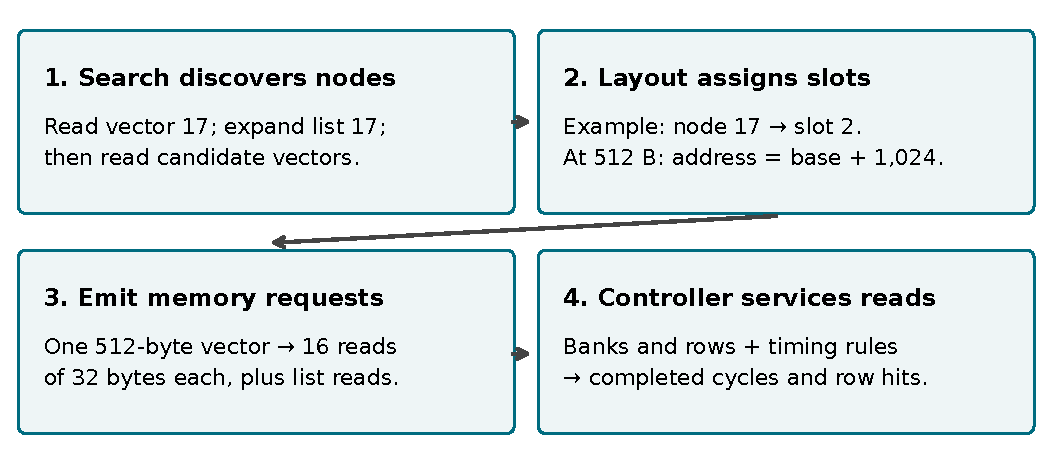
\includegraphics[width=\textwidth]{generated/study_pipeline.pdf}
\caption[The experiment pipeline]{From a graph search to a timing result. Node 17 and slot 2 are an illustrative example, not another measured experiment. Changing the layout changes the second stage while preserving the first.}\label{fig:pipeline}
\end{figure}

For example, suppose the logical search needs vectors 17 and 29 consecutively. One layout might place them in slots 2 and 3, and another in slots 2 and 4. At 512 bytes per vector and a 1-KiB aligned block, slots 2 and 3 share a block; slots 2 and 4 do not. Both searches still evaluate the same vectors and return the same answers. Their memory addresses differ, so the controller may require different commands or expose different bank overlap. This is the intervention the experiment isolates.

\begin{figure}[htbp]\centering
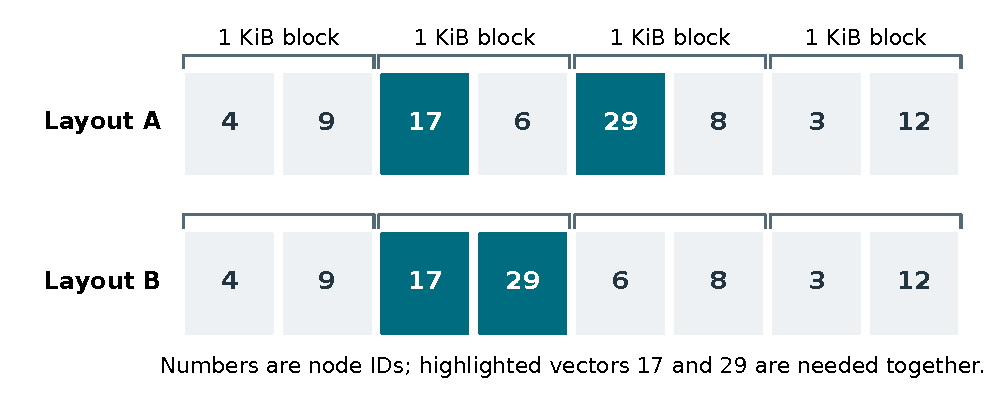
\includegraphics[width=\textwidth]{generated/layout_example.pdf}
\caption[Example of vector placement]{An illustrative excerpt of two vector layouts. Each vector occupies 512 bytes, so two fit in a 1-KiB block. Layout B puts the highlighted pair in one block while retaining every shown vector exactly once. That creates an opportunity for row reuse, but also concentrates the pair's requests in one bank.}\label{fig:layout-example}
\end{figure}

\section{Stock-search instrumentation}
The search implementation is hnswlib \cite{hnswlib}; the artifact identifies the vendored headers and observer changes.
The vendored search implementation contains observer calls immediately before vector distance reads and after determining an expanded list's length. Heap operations, candidate bounds, stopping conditions, and tie handling remain in stock search. The adapter snapshots adjacency for every graph level after construction and forwards observer records to a collector. The observer is cleared after successful and exceptional searches.

The maintained build disables optional CPU prefetching while retaining SIMD distance arithmetic and stock search decisions. Prefetches are speculative early memory requests, outside this demand-stream model. The remediation record documents the vendor safety issue that motivated disabling that implementation path.

Internal HNSW node numbers follow insertion order, while external corpus IDs must remain stable. The adapter translates internal IDs in observed accesses and adjacency lists back to corpus IDs. Tests check that translation against an independently built index after shuffled insertion. Thus changing construction does not silently change the meaning of identity placement or exact-neighbour IDs.

The adapter is single-threaded; the mutable observer is not a general concurrent-search interface. Tests compare results against a separately built stock index on continuous and tie-heavy inputs, with $\texttt{efSearch}=4$ and 64 and $k=10$. They also check entry-vector presence and list sizes. In every real evaluation query, instrumented and unobserved stock result lists must match exactly before the run continues.

Direct instrumentation is stronger than maintaining a second approximate implementation of the search algorithm, but still requires auditing the selected hooks. The instrumentation covers demand vector/list accesses. It does not turn hnswlib into a full CPU memory tracer.

\section{Address representation}
Let $b$ be the vector payload in bytes, $N$ the corpus size, and $B=32$ the native transaction size. Vectors occupy a dense separate array starting at $A_V=\mathtt{0x10000000}$:
\begin{equation}
 a_V(v)=A_V+\pi(v)b,\qquad A_V\leq a_V(v)<A_V+Nb.
\end{equation}
The adjacency region begins at the next transaction boundary after the vector end plus a 1-MiB separating gap. Every $(v,\ell)$ list receives its own aligned allocation in node/level order. Its payload is
\begin{equation}
 s_A(v,\ell)=4+4\,\deg(v,\ell),
\end{equation}
representing a four-byte header and four-byte neighbour IDs. The next list begins after rounding the current allocation end up to $B$. A 32-neighbour base list therefore occupies 132 payload bytes and reserves 160 bytes at 32-byte alignment. Distinct list allocations cannot overlap. The allocation is independent of vector layout for a given footprint.

For any payload beginning at $a$ with size $s$, the emitted transactions cover
\begin{equation}
 B\left\lfloor\frac{a}{B}\right\rfloor,\;B\left\lfloor\frac{a}{B}\right\rfloor+B,\ldots < a+s.
\end{equation}
This handles partial and unaligned payloads. It can read padding or the containing line of a neighbouring dense vector, but does not reuse a fetched line across logical records. There is no cache or duplicate-read coalescing. The two primary vector widths are multiples of 32, so their per-vector request count is layout-independent.

This separate-array representation is not hnswlib's native physical allocation. It isolates vector placement while holding adjacency placement fixed. An integrated reordered index would also need a mapping mechanism; mapping lookup traffic and storage overhead are outside the simulated stream. For non-identity layouts, the artifact stores both mapping directions as 64-bit entries, or $16N$ bytes, excluding container overhead. A deployed implementation could choose another representation, but cannot assume translation is free without justification.

\section{Verified HBM2 geometry}
\label{sec:geometry}
The simulator is the Ramulator 2.1 implementation at the following source revision:
\begin{quote}\small\ttfamily
7bead6cb7c4b03e095c6d4769ae3181a8e0bf6da
\end{quote}
The bibliography cites the Ramulator 2.0 architecture paper and this exact source separately \cite{ramulator,ramsource}. The primary preset is \texttt{HBM2\_8Gb} with \texttt{HBM2\_2000Mbps}. The actual hierarchy is one configured channel, two pseudochannels, two SIDs, four bank groups, four banks, 32,768 rows, and 128 column units. The preset exposes a 128-bit channel interface, but explicitly sets the data payload to 32 bytes for one pseudochannel. The mapper reduces the column count by the prefetch factor of four, giving 32 native transactions per bank-row address span.

The resulting contiguous same-bank, same-row span is $32\times32=1024$ bytes for the default mapper. Its bit decomposition is shown in Table~\ref{tab:bits}. Integration tests send sample addresses through the actual simulator and compare callback addresses with this decomposition, including a high address within the configured capacity. This avoids inferring geometry from a performance curve.

\begin{table}[htbp]\centering
\caption[Default address mapping]{Default \texttt{RoBaRaCoCh} mapping for one channel. Bit 0 is the least significant address bit.}\label{tab:bits}
\begin{tabular}{lrl}\toprule
Field & Address bits & Values\\\midrule
Byte within transaction & 0--4 & 32 bytes\\
Transaction column & 5--9 & 32 columns\\
Pseudochannel & 10 & 2\\
SID & 11 & 2\\
Bank group & 12--13 & 4\\
Bank & 14--15 & 4\\
Row & 16--30 & 32,768\\\bottomrule
\end{tabular}
\end{table}

The alternate \texttt{ChRaBaRoCo} mapper keeps column bits 5--9, places row in bits 10--24, then bank, bank group, SID, and pseudochannel in bits 25--30. It therefore presents very different bank parallelism for a small contiguous range despite retaining a 1-KiB row span. There is no interleaving across multiple configured channels in either experiment.

The preset's DRAM period is 1 ns at its stated 2,000-Mbps transfer rate. Several timing choices in upstream source are annotated as estimates. This work verifies trace interpretation, mapping, and accounting; it does not independently validate the preset against a physical HBM2 device.

\section{Frontend, concurrency, and completion}
\label{sec:frontend}
Each line has the form \texttt{LD address query kind}. The frontend accepts read-only, native-aligned addresses, requires monotonic query positions, and supports untagged microbenchmark lines as one query. It submits at most one transaction per configured issue interval and limits submitted-but-uncompleted requests. A rejected controller submission is retried without advancing the trace.

The controller implementation is \texttt{GenericDDR}, which selects at most one command per controller cycle. The HBM2 timing specification still constrains those commands, but this is not the specialised dual-command-issue HBM controller. This explicit choice limits claims about peak HBM utilisation.

The primary configuration permits 64 outstanding reads, a 32-entry read buffer, and one submission opportunity per memory cycle. These are separate constraints: active and pending controller state can make total in-flight traffic differ from the waiting read-buffer occupancy. The frontend uses completion callbacks to enforce the outstanding limit. The limit counts 32-byte transactions, not vectors: 64 transactions represent 2 KiB of payload, equivalent to four complete 512-byte vectors or sixteen 128-byte vectors before accounting for adjacency traffic. Changing footprint therefore changes both grouping capacity and how much logical vector work fits within this request bound.

At a query boundary, all earlier reads must complete before the next query can issue. Bank-row state remains warm, refresh continues during service, and there is no cache state to reset. The simulation starts with the default initial DRAM state. It terminates only when callbacks have arrived for every trace read. A watchdog rejects a nonterminating run.

The frontend's clock configuration is derived from the pinned simulation loop rather than assumed from parameter names. Its \texttt{clock\_ratio}=1 and the memory system's ratio equal to the issue interval produce one frontend opportunity every specified number of memory cycles. A four-cycle issue interval is tested as a sensitivity.

For each query, the frontend records the minimum accepted-request arrival and maximum read departure in controller cycles. Their difference is the query's stream service interval. Total controller cycles include the complete stream and refresh effects. Neither measure includes graph computations or instruction-level control overhead. The later expansion-bounded experiment adds memory-completion dependencies using the same frontend. An in-flight limit of one serialises memory requests but still does not add distance computation; it is a concurrency sensitivity, not a complete dependency-aware HNSW model.

\section{Page policy and scheduler settings}
The default policy is \texttt{Open}. Sensitivities use \texttt{ClosedCAP} with cap explicitly equal to one and four. A cap is the policy's column-access count within an activation; it is not a guarantee that every pending request is classified as a row miss. The controller can have multiple requests and commands in progress, and upstream row classification occurs when a request is first scheduled. All page-policy findings refer to these implementations.

The study also tests \texttt{FRFCFS-RowHit}, read-buffer capacity eight, outstanding limits one and 16, issue interval four, and the alternate mapper. Every setting first replays all five layouts at both footprints on the first held-out split. Three informative settings---one outstanding read, cap four, and the alternate mapper---are then repeated across all ten splits. The remaining settings retain their exploratory single-split status.

\chapter{Layouts, metrics, and correctness}
With the address representation fixed, the next choice is how to assign nodes to slots. The initial five layouts use progressively different information: corpus order, randomness, graph structure, and observed training searches. This chapter explains those choices and the measurements used to compare them.
\section{Baseline layouts}
\textbf{Identity} assigns slot $v$ to node $v$, preserving corpus order, including when graph insertion is shuffled. It is the practical reference for this separate-array representation, not a claim about the original allocator's addresses.

\textbf{Random} uses a seeded permutation of all nodes. It is a control for locality available from the other mappings, not an upper bound on irregularity. Its RNG varies with the evaluation split seed.

\textbf{BFS} (breadth-first search) visits a node's immediate neighbours before moving to the next graph frontier. It assigns slots in breadth-first order over the base graph, restarting from the lowest unplaced ID for disconnected regions. It may bring some graph neighbours close together, but cannot guarantee that all nodes expanded together share a row.

\textbf{Community} groups nodes by graph connectivity. Each node starts with a label; repeated updates favour labels common among its neighbours. This asynchronous label propagation runs for at most 20 iterations, then places communities contiguously. Community-size ties and within-community choices are deterministic under the configured seed. It is a lightweight structural heuristic rather than an exact graph-partitioning solver.

\section{Workload-trained greedy layout}
The \QA{} method asks which vectors tend to be read near one another during training searches. If nodes 17 and 29 often occur close together in those searches, it gives their pair a larger weight and tries to store them together. This can capture a relationship between two neighbours expanded from the same parent even when the two nodes do not have a direct graph edge. The held-out queries then test whether that training signal is useful beyond the searches used to build it.

Formally, the method learns a symmetric weighted co-visitation graph from training vector accesses. Within a query, each vector access contributes a weight increment with the different nodes in a bounded recent list. The default list capacity is 16 distinct nodes. A node already in that list contributes pairs but is not reinserted or refreshed in recency; the list is therefore a bounded distinct-history heuristic rather than a fixed number of access occurrences. Query boundaries reset the list.

After accumulation, each node's partners are sorted by descending weight, breaking ties by node ID. Seeds are sorted by total incident weight with the same deterministic ID tie-break. The layout places the first unplaced seed and then its heaviest unplaced partners that fit before the current physical block boundary. A short group may leave room for the next seed, but that next seed's partners may not spill into a subsequent block. Unplaced nodes are appended using BFS restarts.

The primary block size is the verified 1,024-byte contiguous row span. A footprint of 512 bytes gives capacity for two complete vectors in an aligned block; 128 bytes gives eight. For example, if a 512-byte block group starts at slot 2, only one partner fits beside the seed before slot 4 begins the next block. At 128 bytes, a fresh aligned block can hold the seed and seven partners. The mapping is rebuilt separately for each footprint. A 2,048-byte grouping is tested as a heuristic sensitivity, without calling it the physical HBM2 row span.

The method optimises a proxy: temporal co-visitation in a finite training sample. It does not know controller command timing or adjacency interference, and does not minimise simulated cycles directly. Low coverage, the weighting rule, greedy ordering, and the grouping objective can each limit its performance. A loss by this method would not prove that the workload has no useful placement information.

\section{Published placement baselines}
The initial five layouts establish the comparison. A follow-up adds RCM, Gorder and Porder using the supplementary implementation of Coleman et al.~\cite{coleman}. This closes a specific comparison gap: a result from one local heuristic cannot represent established graph-reordering methods.

RCM (reverse Cuthill--McKee) runs degree-ordered breadth-first traversal and reverses the resulting order \cite{cuthill,coleman}. Gorder \cite{gorder} greedily places nodes using relationships to a recent placement window: direct graph links and neighbours sharing an incoming parent can both increase a node's score. Porder weights those relationships with observed search traffic. These methods make different approximations to locality; none directly optimises the simulated controller's completion time. We apply the supplied routines to the directed base-layer graph with their five-node Gorder/Porder window, then use the returned permutation for the separate vector array. Upper-layer demands remain in the replay. Adjacency storage remains fixed. This evaluates published placement routines in this thesis's representation; it does not reproduce the authors' native index allocation, caches or application benchmark.

Porder assigns a base-layer edge weight of one plus the number of training searches that evaluate its destination through that edge. The profile uses only the 500 training queries. Evaluations already suppressed by the visited structure do not increment an edge. The local query-aware heuristic instead weights co-visited vector pairs, including pairs without a graph edge, and packs groups according to footprint. The two trained methods therefore use related evidence but different objectives.

The supplied routines and their source archive are hash-pinned. Differential checks compare the adapter with the untouched reference; implementation details and the supplied window convention are in Appendix~\ref{app:adapters}.


\section{Metrics and their meanings}
\subsection{Search accuracy and traffic}
For each test query, exact squared distances are evaluated over exactly the indexed base subset, using double accumulation and distance/ID sorting. Recall is computed against those IDs. Full-million-vector ground truth is not used for the 100k index. The SIFT components have integral values in the mirrored float representation, which also makes the recorded tie convention interpretable.

Vector and adjacency logical records, their graph levels, emitted read count, allocated address bounds, construction times, split membership, returned IDs, and truth IDs are retained. Upper-layer records constitute \UpperFraction\% of logical evaluation records on average. They are included in timing rather than discarded on the assumption that they are negligible.

\subsection{Address-colocation diagnostics}
Let $v_1,\ldots,v_m$ denote one query's vector records in order, after skipping consecutive repeated node IDs for the transition count. For block size $R$, define
\begin{equation}
 g(v)=\left\lfloor\frac{\pi(v)b}{R}\right\rfloor.
\end{equation}
The \emph{consecutive-vector same-block fraction} counts transitions for which $g(v_i)=g(v_{i+1})$, divided by all eligible within-query transitions, then aggregates counts across queries. It compares vector starts, not all bytes of a potentially crossing vector. It resets between queries and ignores adjacency records by definition.

A second diagnostic takes each query's unique visited-node set and counts pairs sharing a start-address block. This co-visit same-block fraction is computed using per-block counts, avoiding explicit quadratic enumeration. Both diagnostics are address statistics. They do not include bank state, intervening adjacency requests, controller reordering, or command timing. They must not be labelled measured DRAM row-hit rates.

\subsection{Simulator outputs}
The primary performance quantity is completed-stream controller cycles. The simulator's read row-hit fraction is
\begin{equation}
 H=\frac{n_{\mathrm{hit}}}{n_{\mathrm{hit}}+n_{\mathrm{miss}}+n_{\mathrm{conflict}}}.
\end{equation}
The three counters classify requests in the pinned controller. They are not an application speedup and need not track cycles monotonically. Raw controller statistics include latency and throughput values, but the thesis's headline comparison uses cycles and conserved traffic, avoiding an inference from a more visually separated proxy.

\section{Maintained checks}
Table~\ref{tab:checks} describes invariants checked by the artifact. Tests target failure modes that can change the scientific comparison; the numerical direction of a layout result is not made a test requirement.
\begin{table}[htbp]\centering\small
\caption[Correctness checks]{Correctness checks required before analysing results.}\label{tab:checks}
\begin{tabular}{p{0.29\textwidth}p{0.62\textwidth}}\toprule
Area & Check\\\midrule
Search & 800 independent-index result comparisons across corpus/shuffled insertion, including ties and $\mathrm{ef}<k$; per-query instrumented/unobserved equality in every real run.\\
Address space & All adjacency levels have separate aligned ranges; known 132-byte lists cannot alias; partial payloads emit every touched transaction.\\
Placement & Every mapping is a bijection with a valid inverse; footprint-specific constructions and partial-group boundaries have regression cases.\\
Metrics & A vector in each of two separate queries cannot create a within-query transition; known same-block examples produce the expected count.\\
Input & Empty, short, ragged, nonfinite and truncated records fail; numeric overflow and negative parameters fail in maintained trace tools.\\
Frontend & Native transaction size and mapper samples match the actual configuration; outstanding limits and query drain are checked; a one-read trace completes.\\
Accounting & Trace lines, submitted reads, completed callbacks, served reads, and classified reads must agree for every analysed run.\\
Quality sweep & Slots remain unique and the address multiset is identical at every quality setting; observed fixed slots match the requested integer count.\\\bottomrule
\end{tabular}
\end{table}

\chapter{Experimental protocol}
A fair comparison needs more than several layout implementations. It needs the same search work, a clear accuracy check, disjoint training and evaluation, and repetitions that vary the intended source of uncertainty. The protocol first tests controlled streams, then actual HNSW demands, and finally the assumptions on which the comparison depends.
\section{Data, construction, and held-out queries}
The SIFT source is the ANN-Benchmarks HDF5 mirror \cite{annbench,pq}. The artifact records its SHA-256 digest, converts the first 100,000 training vectors to fvecs, and converts all 10,000 query vectors. Corpus IDs are the zero-based prefix positions. The mirror calls corpus data ``train'' and query data ``test''; those names are separate from this thesis's training/test partition of the query pool. Query IDs are retained after shuffling; vector dimensions and finite components are checked.

HNSW supplies a widely used graph-search workload with explicit data dependencies and an available stock implementation~\cite{hnsw}. SIFT supplies public, fixed-dimensional data and a reproducible query pool~\cite{annbench}. The 100k prefix keeps exact subset-neighbour verification and the repeated simulation matrix tractable. This is a controlled case study, not a representative sample of modern embedding workloads. With $M=16$, construction search width 200, query search width 64 and $k=10$, it evaluates one high-recall operating point; these settings were not selected by an accuracy/latency sweep.

For each of ten split seeds, a permutation of the fixed 10,000-query pool determines the split. The first 500 queries train the co-visitation model; the last 200 evaluate every layout. This convention keeps the same test queries when training size changes and leaves training and testing disjoint. Repetitions hold the corpus, insertion order, HNSW parameters, and index seed 100 fixed. They vary training/test selection and the random/community layout seeds. They do not quantify index-construction variation or alternative corpus subsets.

Index reconstruction uses the same deterministic insertion protocol in each process. Corpus and trace hashes, parameters, query IDs, and mappings identify the experiment. Results describe this fixed graph and query pool. Additional datasets and search operating points would be required for broader ANN conclusions; selected index constructions are evaluated separately.

\section{Two different kinds of repetition}
A random seed makes a pseudo-random procedure reproducible. It does not specify what source of variation is being tested. The primary ten seeds change which queries train and evaluate a layout, while keeping the graph fixed. The added construction study changes graph seeds to 101 and 102 while retaining corpus order, and separately uses graph seed 100 with shuffled insertion order seeded by 17. Each of these three additional graphs uses query splits one through three. The original graph on those same three splits supplies the reference.

Corpus IDs and the exact-neighbour search universe remain fixed. Layouts are compared within a graph and split; raw times across different graphs also reflect different search work. Graph and insertion-order hashes verify that the intended graph is reused across its splits and that the selected constructions differ. With only three deliberately selected alternatives, their results are reported as observed means and ranges, not as a confidence interval over all possible graphs.

\section{Paired uncertainty}
\label{sec:paired}
For split $s$ and layout $L$, let $T_{s,L}$ be completed-stream cycles at one fixed footprint. The paired relative difference against BFS is
\begin{equation}
 d_{s,L}=100\left(\frac{T_{s,L}}{T_{s,\mathrm{BFS}}}-1\right).
\end{equation}
For example, 99,700 cycles against a 100,000-cycle BFS run gives $d=-0.3\%$: fewer cycles is a negative difference. Each comparison uses the same queries and graph, so a difficult query set cannot make one layout look worse simply because it was tested on more work. The estimate is the mean of these ten differences. The reported interval is
\begin{equation}
 \bar d_L\;\pm\;t_{0.975,9}\frac{s_d}{\sqrt{10}},\qquad t_{0.975,9}\approx2.262,
\end{equation}
using the conventional Student interval \cite{student}. The sampling unit is an independently selected split/layout RNG condition within the fixed pool. The interval expresses uncertainty in the mean effect under this protocol; it is not a range that should contain 95\% of individual query latencies. Query sets may overlap between repetitions; there is no leakage between training and testing within one split. The interval describes variability induced by that random protocol, conditional on the corpus, graph and simulator.

The simulator is deterministic for a fixed trace and configuration; rerunning identical inputs would not measure workload uncertainty. Individual queries are not treated as independent hardware replications, and overlap of marginal layout intervals is not used as a test of a paired difference. These are exploratory 95\% intervals for individual comparisons, without a family-wise multiplicity correction. An interval containing zero is inconclusive about the sign at this precision; it is not evidence of equivalence. No equivalence margin is specified, and the study makes no statistical-equivalence claim.

Ten splits provide a finite estimate of query-selection variability at an affordable simulation cost; ten is not a universal sufficiency threshold. No prospective power calculation or minimum practically useful effect was specified. The reported intervals and individual split effects show the achieved precision for these comparisons. Heavy-tailed split effects would call for more repetitions and an alternative interval check. More splits could refine that conditional mean, but would not test a new dataset, graph family or hardware platform. Robustness across those dimensions requires changing the corresponding experimental input.

\section{Controlled microbenchmarks}
The ordering experiment reads 4,096 vectors with 128-byte payloads, producing 16,384 native transactions. Sequential and permuted variants have identical address multisets. Request presorting stably sorts disjoint batches of 1, 16, 64, 256, 1,024, 4,096, or 16,384 \emph{transaction records}. These are not sliding windows or numbers of vectors. The full-size sort is checked to reproduce the sequential trace byte for byte.

The run-length generator visits contiguous groups in shuffled group order. Run lengths are 1, 2, 4, 8, 16, 32, and 64 vectors. Payload widths are 96, 128, 192, 256, 384, and 512 bytes; base offsets relative to the aligned base are 0, 32, and 480 bytes. A smaller run/mapping matrix also tests the alternate mapper. The generator evaluates available locality, not attainable HNSW placement.

The placement-quality intervention holds the logical contiguous-group visits fixed at 16 vectors per group. For requested quality $q$, exactly $N-\lfloor Nq/100\rfloor$ IDs are selected and their slots cyclically permuted. All other IDs keep their original slot. The special impossible case of exactly one displaced slot is rejected. Thus ``quality'' means fixed \emph{slot} fraction, not fixed row or cluster fraction. The tested percentages are 0, 25, 50, 75, 90, and 100.

\section{Sensitivity and preprocessing cost}
The real-data sensitivity matrix changes one controller setting at a time on split one. Training-size ablations use 100 and 1,000 queries; window ablations use four and 64 distinct-history entries; block-size sensitivity uses 2 KiB. Their test IDs remain the same, and BFS and \QA{} are both replayed at both footprints.

The driver times index construction, training-query collection, co-visitation construction, and each layout build using a steady clock. These are wall-clock observations on a shared execution environment, with other experiment processes potentially active. They establish that preprocessing is nonzero and expose order-of-magnitude costs. They are not controlled hardware throughput benchmarks or a measured amortisation break-even point.

\subsection{Available requests: an expansion-bounded follow-up}
\label{sec:followup-protocol}
Flat replay knows the finished search trace. A cap on outstanding transactions limits how much it offers at once, but can still offer a later expansion before the reads that discovered it have completed. This raises a directly related question: does placement behave differently when the next work is withheld until its preceding memory work completes?

The follow-up introduces \emph{phases}. An adjacency-list payload forms one phase. The candidate vector reads that follow that list form the next. The frontend drains all reads in each phase before accepting the next phase; initial vector reads and graph-level entry reads receive separate phases. Each candidate is checked against its preceding list at the same level. Figure~\ref{fig:phases} illustrates the boundary. The existing draining query marker represents a phase ID, with a separate map back to the original query. No simulator timing rule is changed, and bank-row state remains warm.

\begin{figure}[htbp]\centering
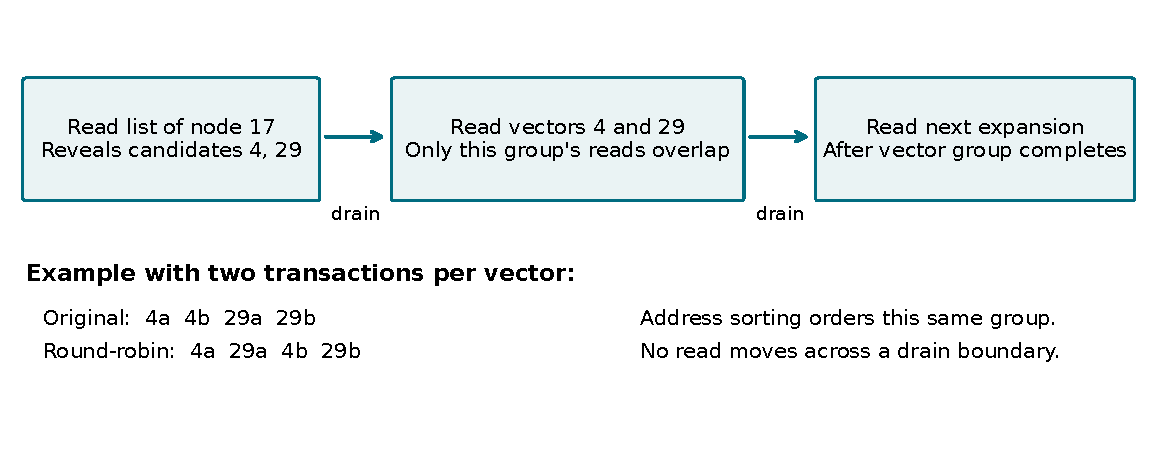
\includegraphics[width=\textwidth]{generated/followup_phases.pdf}
\caption[Requests available within an expansion]{Expansion-bounded replay and two illustrative vector chunks. Real 512-byte and 128-byte vectors contain sixteen and four transactions respectively. An arrow means that earlier reads must complete; computation is not timed.}\label{fig:phases}
\end{figure}

Inside each vector phase, the original transaction order is compared with two schedules. \emph{Address sorting} places the available transactions in ascending address order. \emph{Transaction round-robin} offers the first chunk of each vector, then the second chunk of each, and so on. Sorting aims to bring nearby addresses together; round-robin aims to expose several vectors earlier. Every transaction, including duplicates, remains in its original phase. Neither schedule borrows requests from a later expansion. Their scheduling and buffering costs are omitted, so they measure opportunities before implementation overhead.

The model assumes that the selected candidate vectors within an expansion can be fetched together. It does not implement the search's distance arithmetic or instruction-level control flow, and can expose more intra-expansion overlap than stock execution. Conversely, draining every expansion excludes overlap that a more asynchronous implementation might achieve. It is a defined memory-dependency sensitivity, not a cycle-exact PIM engine or a bound on every implementation.

The fixed design adds 494 replays: 19 graph/split pairs, two footprints, and 13 conditions per pair/footprint. The conditions comprise three published layouts under flat replay; identity, BFS, query-aware and the three published layouts under expansion boundaries; and both alternative schedules on BFS and query-aware placement. The 19 pairs are the ten reference splits plus three splits for each additional construction. The default mapper, open-page controller and 64-transaction limit are unchanged. The original 791 results remain available. The design was recorded before follow-up timings, with no method removed after observing its result. Because the queries were used previously, these are exploratory extensions rather than an independent validation set.

For a bounded query, service begins at the first arrival in its first phase and ends at the last departure in its final phase. Thus the reported interval includes the gaps between phases. Raw phase means are not reported as query means. Placement comparisons match both boundary mode and baseline; schedule comparisons use the same layout with original-order bounded replay. Ten-split intervals remain conditional on the reference graph. Additional constructions are reported separately on matched splits one through three. All layouts are compared with identity and BFS in the retained summaries.

\subsection{Scheduling robustness}
\label{sec:scheduling-protocol}
The default scheduling contrast raises a specific question: how much does it depend on the requests exposed to the controller? Earlier controller sweeps changed flat-replay placement; they do not answer this scheduling question. The final sensitivity matrix therefore compares all three schedules on BFS placement, using the ten reference splits and both footprints.

Six conditions change one assumption at a time. Three set the outstanding-transaction limit to 16, 32 or 128, retaining the 32-entry controller read buffer. Two split each candidate-vector phase into consecutive batches of at most two or eight vectors, draining each batch before the next starts. The last uses the previously evaluated alternative address mapper. All other settings match the default bounded model. This adds 360 replays; the 64-outstanding, full-phase default reuses the earlier evidence. The design was fixed before inspecting these timings, and every condition remains in the results.

\begin{figure}[htbp]\centering
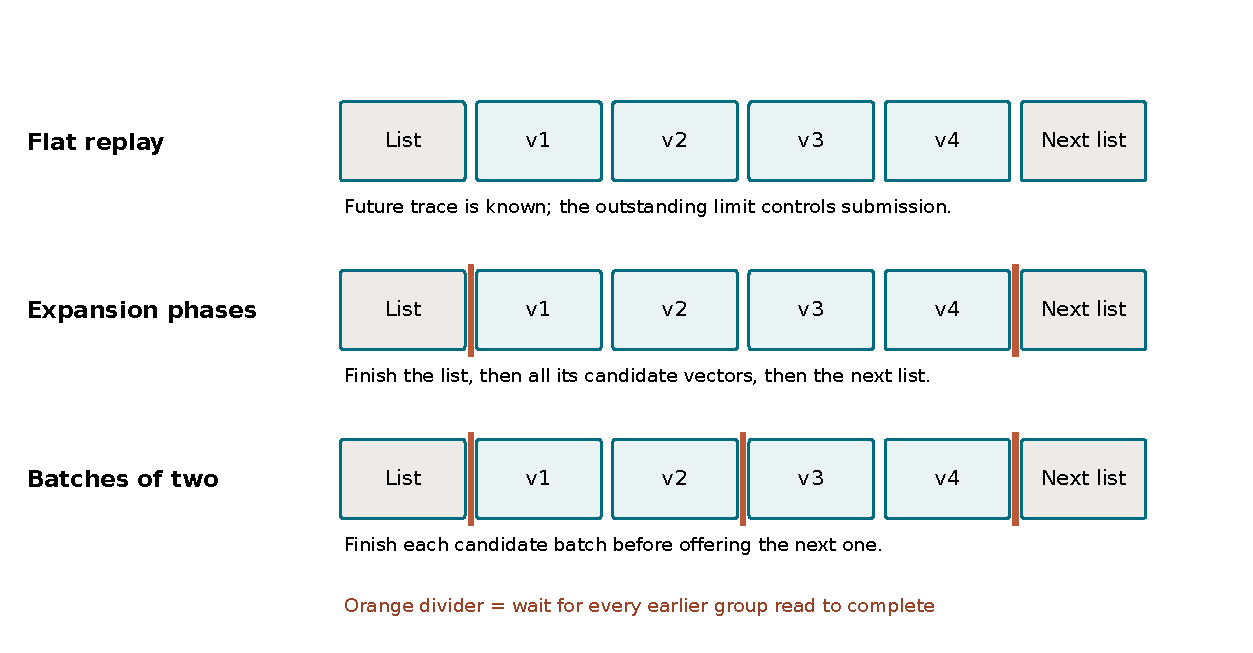
\includegraphics[width=\textwidth]{generated/replay_models.pdf}
\caption[What the replay boundaries mean]{The same illustrative logical sequence under three availability models. Orange dividers require completion of the preceding group. Vector reads inside a group may overlap subject to controller and outstanding limits. Horizontal position denotes request order, not elapsed time. All modes omit computation and integration costs.}\label{fig:replay-models}
\end{figure}

Figure~\ref{fig:replay-models} separates candidate batching from a transaction limit. A batch bounds the vectors whose chunks are offered before a drain; the outstanding limit bounds accepted reads that have not completed. A batch is not a rolling residency limit, and its extra drains can prevent overlap that a different implementation would exploit. Each schedule is compared with original order under exactly the same boundaries. Original-query service includes every inter-batch gap.

The emitter reproduces the previous flat BFS trace hashes before changing order, checks every batch's transaction multiset and retains the parent expansion of each batch. A one-vector batch supplies an exact sanity check: original order, sorting and round-robin produce identical streams. The retained evidence includes losslessly compressed phase timings, source/trace hashes, matched read counts and the complete named matrix. Pairing and confidence intervals follow Section~\ref{sec:paired}; reused queries do not turn this sensitivity study into independent confirmation. Graph-construction variation remains a separate experiment at default scheduling settings.

\subsection{A training-selected vector-fetch path}
\label{sec:profile-protocol}
The scheduling reversals suggest a modest execution proposal: choose how to fetch an expansion's vectors using a short profile of the target configuration. HNSW still chooses which candidates to inspect. The optional path chooses only the order in which their memory transactions are offered. It requires a near-memory engine or frontend that exposes those requests; the experiment does not establish that a particular commercial PIM product provides this interface.

For each reference split, use the first 50 of its 500 training queries. Replay their BFS vector placement with original order, address sorting and transaction round-robin under the target configuration. Select the order with minimum total completed service cycles; exact ties prefer original order, then sorting, then round-robin. Store that choice once and use it for all 200 held-out queries. This is a configuration-level choice, not a decision made using each test query's outcome. The training and test IDs are disjoint within every split.

The profile is specific to the graph/layout, footprint, batch limit, outstanding bound and memory configuration. It selects only request order; it does not choose a layout, batch size or hardware configuration. The experiment repeats it for the default and six sensitivity conditions at both widths, producing 140 choices from 420 calibration replays. The selected order's held-out request stream has already been measured in the scheduling campaigns; evaluation uses that exact record. Calibration runs are additional training evidence, not additional independent performance repetitions.

This extension was designed after inspecting early sensitivity reversals and previously evaluated test outcomes. Its 50-query budget, three choices and tie rule were then fixed in \texttt{doc/PROFILED\_FETCH\_DESIGN.md}; all outcomes are retained. Although selection code reads training costs only, the overall study remains exploratory because those observations motivated the policy and queries recur across splits. An untouched workload would be needed for a stronger generalisation claim.

Compare the selected path with every fixed schedule under matching settings. Also report its difference from the retrospectively best fixed schedule on each held-out split. That \emph{oracle} is a descriptive reference: it uses test outcomes and is unavailable to a deployed selector. At default settings, compare with the measured RCM, Gorder and Porder placements using original order. Those are whole-configuration comparisons; combining published placements with the selector is a separate, unevaluated intervention. Report profiling service cost separately from held-out savings. No inference about application amortisation follows without implementation costs in common units.


\chapter{Results}
\label{ch:results}
The results follow the argument from a simple case to recorded graph-search demands. Controlled streams first reveal why locality and timing can disagree. The SIFT experiment then measures how much the tested layouts change service at fixed search work. Repeated controller settings, graph variations and command diagnostics examine how stable those differences are and why they arise.
\section{Ordering: row hits and cycles can disagree}
Figure~\ref{fig:order} begins with the simplest controlled comparison: two orders of the same reads. Sequential service takes \SequentialCycles{} cycles at \SequentialHit\% classified row hits. The permuted stream takes \RandomCycles{} cycles at \RandomHit\% hits. Every stream read completes and is represented in the classification counters.

The sequential sequence has a higher hit fraction but takes more cycles at the default concurrency. This result is compatible with the different banks exposed by the request order: with the default mapping, 32 adjacent transactions fill one row span, so a 64-request contiguous prefix exposes only two bank instances, whereas scattered vectors can expose more. The exact performance follows from scheduling, buffers, and timing together. Row-hit fraction alone does not isolate the cause or establish a necessary condition for good service.

At outstanding limit one, full sorting changes the permuted stream's 398,592 cycles to 325,786 cycles. This comparison is retained in the raw sensitivity results and demonstrates that available concurrency materially changes the ordering result. It does not add HNSW's compute dependencies.

\begin{figure}[htbp]\centering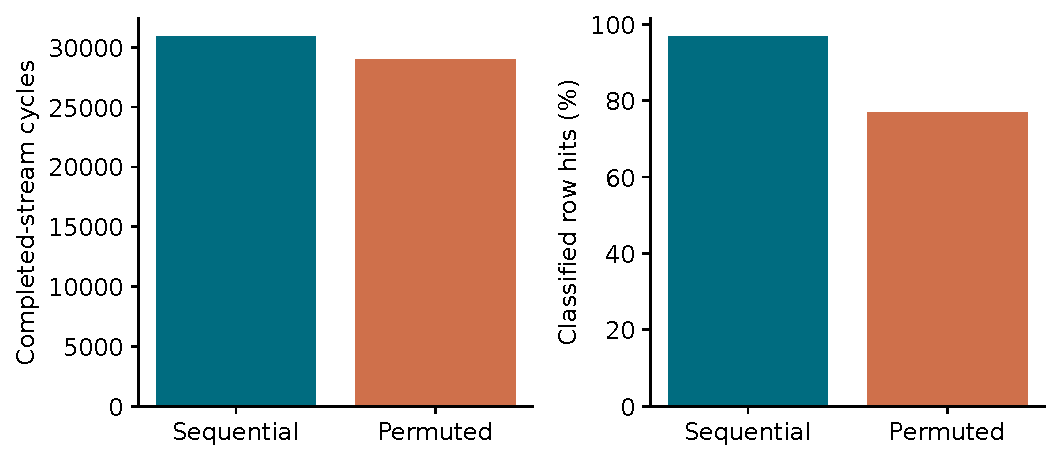
\includegraphics[width=\textwidth]{generated/micro_order.pdf}
\caption[Row hits and service cycles]{Default native-transaction microbenchmark. Higher row-hit fraction does not imply fewer completed-stream cycles.}\label{fig:order}\end{figure}

\subsection{Following the commands rather than the proxy}
The next step is to ask what the controller actually does. The pinned simulator provides observers that count each issued command and, for the microbenchmark, record its cycle and decoded address. Replaying with these observers gives exactly the same cycles and row-hit counts as the original runs. The observers add evidence without changing the simulated schedule.

Table~\ref{tab:microcommands} gives an exact accounting for this controller. Because it selects at most one command per cycle,
\begin{equation}
 T = N_{\text{command cycles}} + N_{\text{no-command cycles}}.
\end{equation}
A command cycle may open or close a row, issue a read, or perform refresh. A no-command cycle can arise from timing restrictions, a lack of eligible work, or draining the last reads. It is deliberately not labelled as a particular stall cause.

\begin{table}[htbp]\centering\small
\caption[Command accounting for request order]{Controlled ordering experiment with command observers. ACT opens a row; PRE combines per-bank and all-bank precharge commands. The read count is 16,384 in every row. ``Limit'' is the maximum number of outstanding reads.}\label{tab:microcommands}
\begin{tabular}{rlrrrr}
\toprule
Limit & Order & Cycles & ACT & PRE & No command \\
\midrule
64 & Sequential & 30894 & 528 & 38 & 13930 \\
64 & Permuted & 28968 & 3793 & 3319 & 5458 \\
1 & Sequential & 325786 & 588 & 166 & 308482 \\
1 & Permuted & 398592 & 4044 & 1135 & 376825 \\
\bottomrule
\end{tabular}

\end{table}

At limit 64, the permutation opens and closes more rows, yet has fewer no-command cycles. The reduction in those cycles exceeds the cost of the extra command-issue cycles. At limit one, no other read can hide the waiting for the current read, and the additional row changes make permutation slower. The two interventions expose the trade-off: reducing commands and overlapping service are different ways to reduce time.

The offered sequential stream spans an average of \SequentialBanks{} different bank instances per sliding window of 64 requests, compared with \RandomBanks{} for the permutation. Each statistic counts complete windows within queries under the verified default mapper. This measures diversity in the input stream; it is not a measurement of how many banks are ready simultaneously, or how many requests occupy the controller queue.

\begin{figure}[htbp]\centering
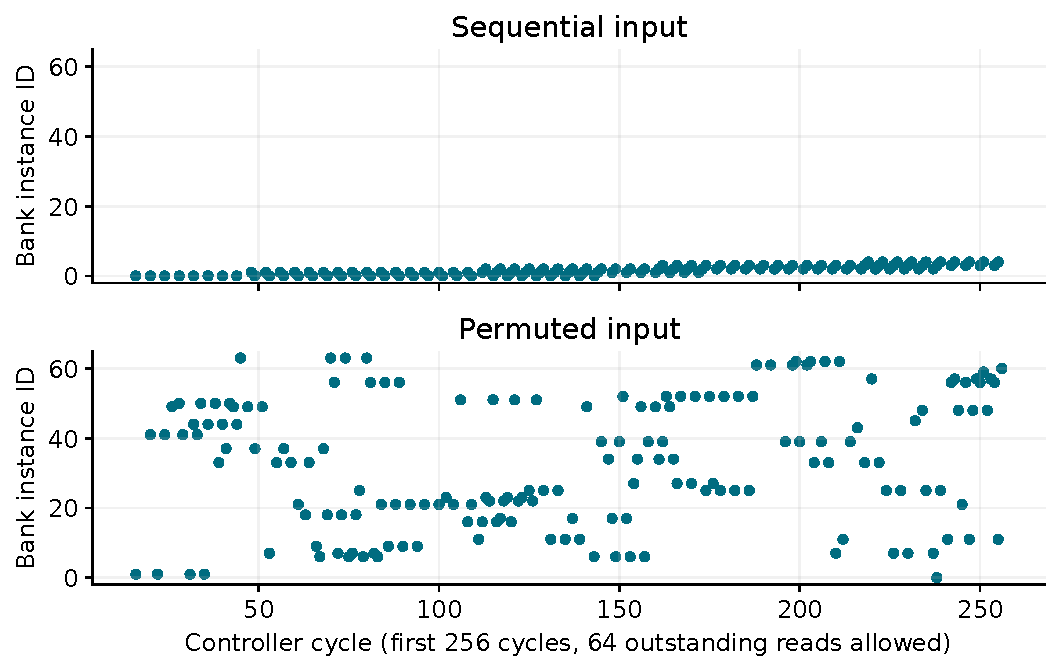
\includegraphics[width=\textwidth]{generated/command_timeline.pdf}
\caption[Read-command timing and bank exposure]{Actual read-command issues in the first 256 controller cycles, with limit 64. Each dot is one RD command; the vertical position identifies its bank instance. Sequential requests concentrate early service in a few banks, while the permutation exposes a wider set. The full-run counts, rather than this short initial interval alone, support the timing comparison.}\label{fig:commands}
\end{figure}

This evidence supports a locality--parallelism explanation for the controlled reversal. It does not assign every saved cycle to an individual timing rule: refresh, buffering and scheduling interact. The important result is that an observed reduction in row operations can be outweighed by the service opportunities lost elsewhere in the schedule.


\section{Finite request presorting}
\begin{table}[htbp]\centering\caption[Request-presorting windows]{Disjoint presorting windows on the permuted 16,384-request trace. The full window exactly reproduces the sequential trace.}\label{tab:reorder}
\begin{tabular}{lrr}
\toprule
Window (requests) & Cycles & Hit (\%) \\
\midrule
1 & 28968 & 76.85 \\
16 & 28950 & 76.92 \\
64 & 28961 & 76.90 \\
256 & 28912 & 77.15 \\
1024 & 28728 & 79.80 \\
4096 & 27001 & 88.70 \\
16384 & 30894 & 96.78 \\
\bottomrule
\end{tabular}
\end{table}
Table~\ref{tab:reorder} reports the tested windows. Sorting can expose a different issue order than the original permutation, and can also reduce bank diversity. Sorting the whole known stream places its addresses in exactly the sequential order; the byte-for-byte trace check verifies this endpoint. Its feasibility during an actual dependent graph search is a separate question: the required future addresses may not yet be known.

The artifact also repeats selected windows with explicit row-hit-prioritising scheduling and with one outstanding request. Those experiments test the controller explanation rather than presuming that all software sorting duplicates FRFCFS. They do not justify a general claim that software reordering is useless or that the largest sorting window is useful in a deployed ANN implementation.

The controlled run-length, alignment and placement-perturbation sweeps provide supporting evidence about how locality is exposed. Their detailed curves and finite-grid thresholds are retained in Appendix~\ref{app:controls}. They do not establish a universal row-size rule or a reusable ANN placement algorithm. The next comparison tests actual graph-search demands.

\section{Held-out SIFT comparison}
Table~\ref{tab:real} contains the real timing comparison and both locality measures. Mean Recall@10 is \SiftRecall\%, with the split-level interval [\SiftRecallLow, \SiftRecallHigh]\%. Within a split all five layouts have exactly the same logical query result and the same emitted read count at a given footprint. The table's differences therefore reflect the modelled placement and controller interactions rather than a changed number of HNSW distance evaluations.

\begin{table}[htbp]\centering\small
\caption[Paired SIFT layout comparison]{Ten paired SIFT100k splits. Cycles are mean totals for 200 held-out queries. Hit is the simulator classification fraction; block is the consecutive-vector same-block diagnostic. The final column is mean relative cycle difference and its paired 95\% interval; negative is faster than BFS.}\label{tab:real}
\resizebox{\textwidth}{!}{\begin{tabular}{lrrrrr}
\toprule
Bytes & Layout & Cycles ($10^6$) & Hit (\%) & Block (\%) & $\Delta$ vs. BFS (\%) \\
\midrule
512 & Identity & 6.2322 & 93.24 & 0.02 & +0.30 [+0.24, +0.36] \\
512 & Random & 6.2327 & 93.24 & 0.00 & +0.31 [+0.12, +0.49] \\
512 & BFS & 6.2138 & 93.40 & 0.77 & +0.00 [+0.00, +0.00] \\
512 & Community & 6.2233 & 93.26 & 0.03 & +0.15 [+0.01, +0.29] \\
512 & Query-aware & 6.1943 & 93.62 & 1.02 & -0.31 [-0.37, -0.26] \\
128 & Identity & 1.6051 & 74.69 & 0.10 & +2.68 [+2.60, +2.76] \\
128 & Random & 1.6089 & 74.54 & 0.01 & +2.92 [+2.80, +3.04] \\
128 & BFS & 1.5632 & 76.47 & 1.68 & +0.00 [+0.00, +0.00] \\
128 & Community & 1.6000 & 74.83 & 0.21 & +2.35 [+2.17, +2.53] \\
128 & Query-aware & 1.5659 & 77.85 & 4.12 & +0.17 [+0.11, +0.24] \\
\bottomrule
\end{tabular}
}
\end{table}
\begin{figure}[htbp]\centering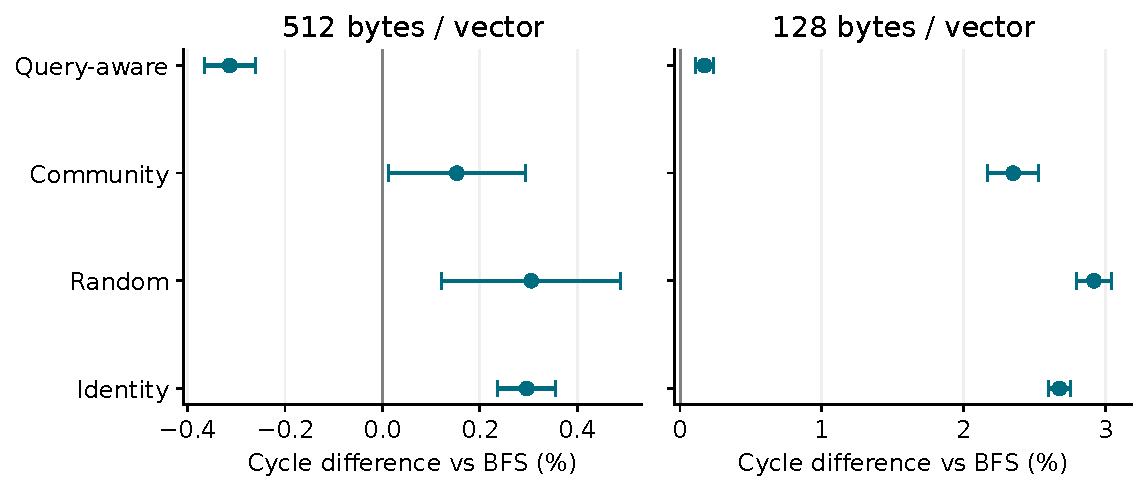
\includegraphics[width=\textwidth]{generated/real_paired.pdf}
\caption[Paired layout differences and uncertainty]{Paired cycle differences relative to BFS. Intervals describe query-split and random-layout variability on a fixed corpus/index/model.}\label{fig:paired}\end{figure}

For 512-byte vectors the \QA{} difference is \QADeltaFloat\% [\QALowFloat, \QAHighFloat]; for the hypothetical 128-byte footprint it is \QADeltaCompact\% [\QALowCompact, \QAHighCompact]. The footprint-specific mapping is rebuilt to match the number of vectors that fit in each grouping block. However, the 128-byte case still retains float32 traversal and recall. Its result cannot be promoted to evidence about PQ accuracy, quantised traversal, or distance-kernel speed.

The pairing matters because query difficulty changes the total traffic and cycles across splits. Comparing layout totals from unrelated query sets would confound the intervention. The original layout is included because a gain over a random permutation alone does not establish a benefit relative to the storage order available to a user.

The single-split controller and training sweeps are retained in Appendix~\ref{app:exploratory}. They identify conditions worth repeating but do not carry the same statistical weight as the paired ten-split results below.

\section{Repeating the controller comparisons}
The exploratory matrix identifies informative changes, but a single split cannot show their variability across query samples. We therefore repeat three settings on all ten primary splits: one outstanding read, ClosedCAP cap four, and the alternate address mapper. These change the opportunity for overlap, row lifetime and address-to-bank placement respectively. Each setting replays all five layouts at both footprints, for 300 additional runs.

\begin{table}[htbp]\centering\small
\caption[Repeated controller comparisons]{Query-aware cycle difference against BFS under three repeated controller settings. Each estimate uses ten matched splits with the same graph. Negative means fewer cycles.}\label{tab:repeated}
\begin{tabular}{lrrr}
\toprule
Setting & Bytes & $\Delta$ QA/BFS (\%) & 95\% interval \\
\midrule
Outstanding: 1 & 512 & -0.13 & [-0.14, -0.13] \\
Outstanding: 1 & 128 & -1.26 & [-1.30, -1.21] \\
ClosedCAP, cap 4 & 512 & +0.89 & [+0.79, +0.99] \\
ClosedCAP, cap 4 & 128 & +5.27 & [+5.15, +5.39] \\
Alternate mapper & 512 & -4.02 & [-4.28, -3.75] \\
Alternate mapper & 128 & -4.12 & [-4.26, -3.99] \\
\bottomrule
\end{tabular}

\end{table}
\begin{figure}[htbp]\centering
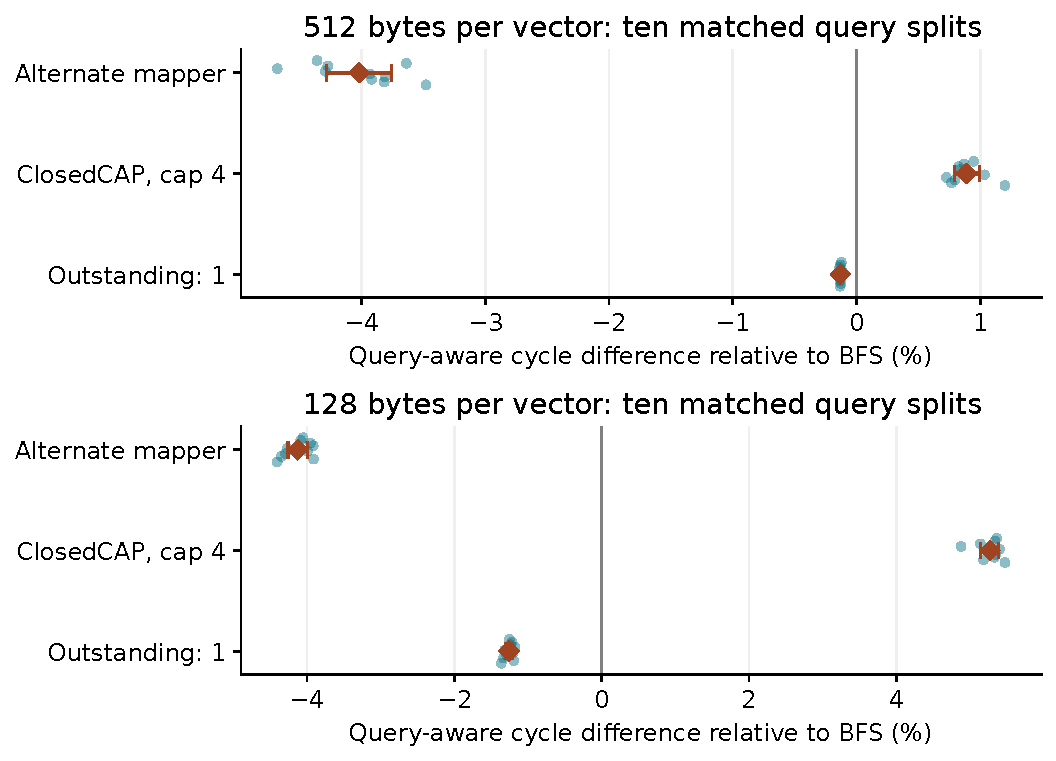
\includegraphics[width=\textwidth]{generated/robust_controllers.pdf}
\caption[Individual effects and paired intervals]{Individual split effects (small teal points) and mean with paired 95\% interval (orange diamond and bar). Showing the observations alongside the intervals makes their consistency and dispersion visible.}\label{fig:repeated}
\end{figure}

The query-aware/BFS sign is consistent across all ten splits in each repeated setting: query-aware is faster at both widths with one outstanding read and with the alternate mapper, and slower at both widths under cap four. The size of the effect also changes substantially, as Table~\ref{tab:repeated} shows. Under the alternate mapper, random placement is faster still than query-aware at 512 bytes in every split. A gain relative to BFS therefore does not identify the best layout among all controls.

The other controller settings and all training ablations retain their single-split interpretation. The repeated settings were chosen after inspecting the exploratory matrix; their ten splits include that original first split. This is a targeted robustness extension, not an independent confirmatory experiment. It strengthens the comparison under those specific interventions without sampling an architectural population.

\section{Changing the graph while preserving corpus IDs}
The previous repetitions share one constructed graph. The next experiment keeps the same 100,000 vectors but changes the structure used to search them. Graph seeds 101 and 102 vary HNSW's random construction with corpus insertion order fixed. A third alternative keeps graph seed 100 and shuffles insertion with seed 17. Each alternative uses query splits one through three and all five layouts at both footprints, adding 90 replays.

\begin{table}[htbp]\centering\small
\caption[Graph-construction robustness]{Query-aware/BFS cycle differences for four constructions on the same three query splits. The mean and minimum/maximum describe these observations; the range is not a confidence interval over possible graphs.}\label{tab:graphrobust}
\begin{tabular}{lrrr}
\toprule
Graph construction & Bytes & Mean $\Delta$ (\%) & Observed range (\%) \\
\midrule
Seed 100, corpus order & 512 & -0.341 & [-0.357, -0.331] \\
Seed 100, corpus order & 128 & +0.119 & [+0.034, +0.186] \\
Seed 101, corpus order & 512 & -0.247 & [-0.386, -0.062] \\
Seed 101, corpus order & 128 & -0.191 & [-0.267, -0.081] \\
Seed 102, corpus order & 512 & -0.268 & [-0.330, -0.212] \\
Seed 102, corpus order & 128 & -0.705 & [-0.798, -0.627] \\
Seed 100, shuffled order & 512 & -0.320 & [-0.499, -0.161] \\
Seed 100, shuffled order & 128 & +0.040 & [-0.057, +0.203] \\
\bottomrule
\end{tabular}

\end{table}

Under flat replay at 512 bytes, query-aware placement uses fewer cycles than BFS in every tested construction/split pair. At 128 bytes, the ranking changes: the reference graph's three-split mean is \GraphRefCompact\%, while seeds 101 and 102 give \GraphOneCompact\% and \GraphTwoCompact\%. Shuffled insertion has mean \GraphShuffleCompact\% and individual splits on both sides of zero. Thus the original 128-byte loss is not a stable property of the footprint alone. Query-split precision on one graph did not establish robustness to constructing another graph.

The reference row uses only those same three splits, making it comparable with the alternatives. Graph hashes confirm four distinct topologies, and repeated builds of each construction agree. Corpus IDs remain stable: changing insertion order does not redefine which vector a logical ID names, which vectors count as exact neighbours, or what identity placement means.

Recall across these graph/split conditions ranges from \GraphRecallMin\% to \GraphRecallMax\%. A changed graph can change the number of candidate evaluations and therefore total traffic. For this reason, Table~\ref{tab:graphrobust} compares layouts within each graph and split. Directly comparing absolute cycles from two different graphs would combine search-work and placement effects. These selected constructions expand the evidence beyond one topology, while leaving corpus and dataset generalisation open.

\section{Explaining the 128-byte layout reversal}
The main SIFT table contains a smaller version of the controlled paradox: query-aware placement gives more row hits than BFS at 128 bytes, yet slightly more cycles. To inspect that result, the command observers replay split one for both layouts with outstanding limits one and 64. Each case is run with the original mixed trace, vector requests only, and adjacency requests only. Query boundaries are preserved. Removing a request type is a diagnostic intervention, not an alternative complete HNSW execution.

\begin{table}[htbp]\centering\small
\caption[Command accounting for the layout reversal]{Query-aware minus BFS for the 128-byte diagnostic streams on split one. Negative counts mean fewer cycles or commands. The last two columns sum exactly to the cycle difference. Limit is the outstanding-read bound.}\label{tab:realcommands}
\begin{tabular}{rlrrrr}
\toprule
Limit & Stream & $\Delta$ cycles & $\Delta$ ACT & $\Delta$ commands & $\Delta$ no cmd. \\
\midrule
64 & Mixed & +2848 & -12516 & -25125 & +27973 \\
64 & Vectors & +3858 & -12401 & -24873 & +28731 \\
64 & Adjacency & +0 & +0 & +0 & +0 \\
1 & Mixed & -278960 & -12771 & -17009 & -261951 \\
1 & Vectors & -265883 & -12582 & -16435 & -249448 \\
1 & Adjacency & +0 & +0 & +0 & +0 \\
\bottomrule
\end{tabular}

\end{table}

For the mixed stream at limit 64, query-aware placement needs \MixedSavedACT{} fewer activations and \MixedSavedCommands{} fewer command-issue cycles. It nevertheless adds \MixedExtraNoCommand{} no-command cycles, leaving a net cost of \MixedDeltaCycles{} cycles. The vector-only case retains the reversal. The adjacency-only traces have the same addresses and order for both layouts and give identical results. Consequently, the effect is already present in vector service; it does not require a changed adjacency layout.

The vector placement also changes offered bank diversity: the mixed input spans \BfsOfferedBanks{} banks per complete 64-request window for BFS and \QAOfferedBanks{} for query-aware placement, on average. This is consistent with increased concentration accompanying row reuse. The observed command/no-command accounting establishes where the cycle difference lies; the input statistic and controlled concurrency experiment support the mechanism, without proving that bank diversity is its only cause.

Vector-only and adjacency-only times must not be added to predict mixed timing. Interleaving the streams changes which requests compete, which rows remain open and which timing delays overlap. The additive identity in Table~\ref{tab:realcommands} applies to command and no-command cycles of a single replay, not to separate component replays.

\subsection{Why a high hit percentage needs a denominator}
A 512-byte vector becomes sixteen consecutive 32-byte reads. In an illustrative uninterrupted access with a closed row initially, one read may require opening the row and the remaining fifteen may hit it: $15/16=93.75\%$. At 128 bytes, the analogous fraction is $3/4=75\%$. These are opportunities within one vector; they are not measured predictions because controller ordering, row state and intervening traffic can change classification.

\begin{table}[htbp]\centering\small
\caption[Within-vector and adjacency traffic]{Traffic composition averaged over the ten primary splits. The last two percentages use all emitted transactions as denominator. A within-vector follow-up is any transaction after the first transaction of that logical vector read. It is not automatically a row hit.}\label{tab:traffic}
\begin{tabular}{rrrr}
\toprule
Vector bytes & Reads/vector & Vector traffic (\%) & Within-vector follow-ups (\%) \\
\midrule
512 & 16 & 98.64 & 92.48 \\
128 & 4 & 94.78 & 71.09 \\
\bottomrule
\end{tabular}

\end{table}

The layout heuristic attempts to improve relationships between different vectors. Table~\ref{tab:traffic} shows why its effect can be small beside the locality already available inside each vector. Reporting the aggregate row-hit rate alone obscures that distinction. The consecutive-vector same-block diagnostic examines another denominator---transitions between distinct vector reads---and therefore cannot be substituted for the simulator's request-based percentage.


\section{Published layouts and requests available within an expansion}
\label{sec:followup-results}
The earlier results leave two natural questions. Would established placement methods do better than the local heuristic? And does their ranking depend on offering future graph work before its preceding reads finish? The follow-up tests both questions while preserving the original experiments. Its comparisons use the default controller; the previously reported policy and mapper sweeps remain supporting evidence for that controller choice's importance.

\subsection{The cost of restricting future work}
Table~\ref{tab:barriers} shows the scale of the memory-boundary intervention. There are \MeanPhasesPerQuery{} phases per query on average on the reference graph, and \MeanVectorsPerPhase{} vectors per vector phase. These are properties of the recorded search at this operating point, not architecture constants. The bounded model gives a different service time because it withholds later work until the preceding phase drains. A global outstanding limit alone does not represent that dependency.

\begin{table}[htbp]\centering\small
\caption[Effect of expansion boundaries]{Reference graph, ten splits. Query service intervals include gaps between phases. The final column is the paired completed-stream difference with a 95\% interval, comparing bounded with flat replay of the same layout.}\label{tab:barriers}
\resizebox{\textwidth}{!}{\begin{tabular}{lrrrr}
\toprule
Bytes & Layout & Flat cycles/query & Bounded cycles/query & $\Delta$ stream (\%) \\
\midrule
512 & Identity & 31,161 & 39,871 & +27.96 [+27.71, +28.20] \\
512 & BFS & 31,069 & 39,811 & +28.14 [+27.88, +28.40] \\
512 & Query-aware & 30,972 & 39,727 & +28.27 [+28.00, +28.55] \\
128 & Identity & 8,025 & 15,874 & +97.81 [+97.06, +98.57] \\
128 & BFS & 7,816 & 15,768 & +101.75 [+100.91, +102.59] \\
128 & Query-aware & 7,830 & 15,783 & +101.60 [+100.80, +102.39] \\
\bottomrule
\end{tabular}
}
\end{table}

These boundaries are not added arithmetic time. They change when requests become available. Bounded timing remains incomplete as an application model: candidate reads in a phase can overlap subject to the outstanding limit, while computation, local buffering and scheduler costs are omitted. A flat/bounded comparison is therefore a sensitivity to execution assumptions, not a measured host/PIM comparison.

\subsection{Placement against stronger baselines}
Table~\ref{tab:followup-layouts} compares all six follow-up placements with BFS under matching boundaries, and with identity under bounded replay. Figure~\ref{fig:followup-layouts} makes the change of scale and ranking easier to see. The prior random and community results remain in Table~\ref{tab:real} and the artifact; they were not part of this prespecified follow-up matrix.

\begin{table}[htbp]\centering\small
\caption[Published and local placement comparisons]{Reference graph, ten paired splits. Entries are mean cycle differences and 95\% intervals; negative values mean fewer cycles. Each baseline uses the same footprint and boundary mode.}\label{tab:followup-layouts}
\resizebox{\textwidth}{!}{\begin{tabular}{lrrrr}
\toprule
Bytes & Layout & Flat / BFS (\%) & Bounded / BFS (\%) & Bounded / identity (\%) \\
\midrule
512 & Identity & +0.30 [+0.24, +0.36] & +0.15 [+0.10, +0.20] & +0.00 [+0.00, +0.00] \\
512 & BFS & +0.00 [+0.00, +0.00] & +0.00 [+0.00, +0.00] & -0.15 [-0.20, -0.10] \\
512 & Query-aware & -0.31 [-0.37, -0.26] & -0.21 [-0.27, -0.15] & -0.36 [-0.43, -0.29] \\
512 & RCM & -0.08 [-0.12, -0.04] & -0.16 [-0.21, -0.11] & -0.31 [-0.35, -0.27] \\
512 & Gorder & -0.29 [-0.35, -0.23] & -0.20 [-0.24, -0.16] & -0.35 [-0.38, -0.32] \\
512 & Porder & -0.55 [-0.68, -0.42] & -0.38 [-0.47, -0.28] & -0.53 [-0.63, -0.42] \\
128 & Identity & +2.68 [+2.60, +2.76] & +0.67 [+0.59, +0.76] & +0.00 [+0.00, +0.00] \\
128 & BFS & +0.00 [+0.00, +0.00] & +0.00 [+0.00, +0.00] & -0.67 [-0.75, -0.59] \\
128 & Query-aware & +0.17 [+0.11, +0.24] & +0.10 [+0.01, +0.18] & -0.58 [-0.64, -0.51] \\
128 & RCM & -0.16 [-0.19, -0.12] & -0.47 [-0.55, -0.38] & -1.13 [-1.19, -1.07] \\
128 & Gorder & -2.79 [-2.84, -2.73] & -1.33 [-1.42, -1.25] & -1.99 [-2.05, -1.94] \\
128 & Porder & -2.47 [-2.57, -2.38] & -1.19 [-1.33, -1.04] & -1.85 [-2.00, -1.70] \\
\bottomrule
\end{tabular}
}
\end{table}
\begin{figure}[htbp]\centering
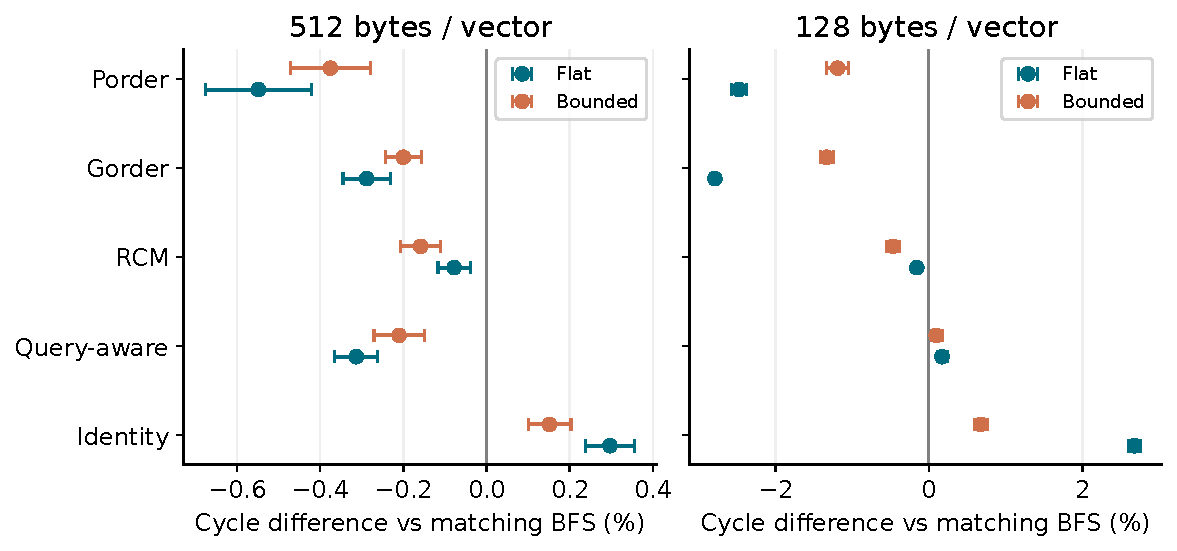
\includegraphics[width=\textwidth]{generated/followup_layouts.pdf}
\caption[Placement under flat and bounded replay]{Layout differences relative to matching BFS, with split-level 95\% intervals. The panels use different horizontal scales. The 128-byte representation is hypothetical.}\label{fig:followup-layouts}
\end{figure}

On the reference graph with expansion boundaries, Porder's cycle difference relative to BFS is \PorderBoundedFloat\% at 512 bytes, compared with \QABoundedFloat\% for the local query-aware heuristic. At 128 bytes, Gorder gives \GorderBoundedCompact\%, while the local heuristic gives \QABoundedCompact\%. These comparisons show why stronger baselines matter: a local heuristic's weak result does not exhaust the available placement improvements.

Porder and the local query-aware heuristic must not be treated as interchangeable implementations of one idea. Their training relationships and placement objectives differ. A weak result for the local heuristic cannot establish that query-guided placement fails in general. Conversely, a gain by a published method in this replay does not reproduce its authors' application-speedup claim. The complete numerical comparisons, including flat replay against identity, are retained in \texttt{results/followup\_summary.csv}.

\subsection{Ordering only the currently available vector reads}
Figure~\ref{fig:followup-schedules} and Table~\ref{tab:followup-schedules} compare address sorting and transaction round-robin with original-order bounded replay on the same placement. The comparison changes order alone: each phase contains exactly the same multiset of transactions. Saved cycles per original query put the relative effect beside an absolute service-time allowance before any scheduling overhead.

\begin{table}[htbp]\centering\small
\caption[Within-expansion request schedules]{Reference graph, ten paired splits. Each schedule is compared with original-order bounded replay of the same layout. Negative percentage differences and positive saved-cycle counts favour the schedule.}\label{tab:followup-schedules}
\resizebox{\textwidth}{!}{\begin{tabular}{lrrrr}
\toprule
Bytes & Layout & Schedule & $\Delta$ cycles (\%) & Saved cycles/query \\
\midrule
512 & BFS & Sorted & +0.19 [+0.13, +0.24] & -74.5 \\
512 & BFS & Round-robin & -14.58 [-14.64, -14.51] & +5802.4 \\
512 & Query-aware & Sorted & +1.79 [+1.75, +1.84] & -712.5 \\
512 & Query-aware & Round-robin & -14.20 [-14.25, -14.15] & +5640.2 \\
128 & BFS & Sorted & +0.17 [+0.12, +0.21] & -26.1 \\
128 & BFS & Round-robin & +3.43 [+3.31, +3.55] & -540.5 \\
128 & Query-aware & Sorted & +1.00 [+0.91, +1.09] & -157.7 \\
128 & Query-aware & Round-robin & +3.30 [+3.21, +3.40] & -521.6 \\
\bottomrule
\end{tabular}
}
\end{table}

\begin{figure}[htbp]\centering
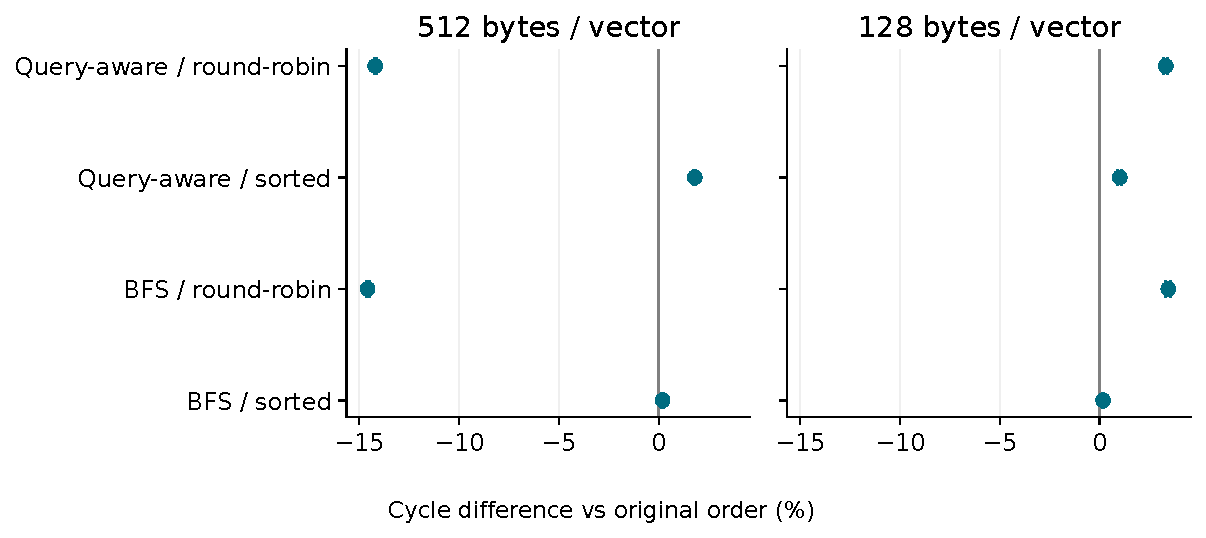
\includegraphics[width=\textwidth]{generated/followup_schedules.pdf}
\caption[When available-request schedules help or hurt]{Mean cycle differences and 95\% intervals on the reference graph. Both panels share the same scale. Every point compares a schedule with original-order bounded replay on the same layout; values left of zero favour the schedule.}\label{fig:followup-schedules}
\end{figure}

The two widths expose different amounts of logical work through a 64-transaction limit. Sixteen chunks belong to one 512-byte vector, but only four to a 128-byte vector. Round-robin exposes several vectors' chunks earlier instead of submitting every chunk of one vector first. This can improve the distribution of offered work, but can also disrupt useful row reuse. Sorting pursues nearby addresses and can have the opposite effect on bank diversity. Neither choice is automatically beneficial.

The per-query check uses the same reconstructed original-query service intervals. For BFS round-robin at 512 bytes, \RRFasterQueriesFloat\% of query records improve in each of the 19 graph/split cases. The within-case empirical 95th-percentile service difference ranges from \RRPtailRangeFloat\%. These are descriptive checks on sets of 200 queries; query IDs can recur between splits, and these records are not additional independent replications. They are service-time observations, not application latency guarantees.

\subsection{Explaining the scheduling contrast}
Four diagnostic replays add command recording to the first reference split's BFS original and round-robin streams at both widths. These repeats were selected after the pilot to explain its contrast; they are not independent statistical observations. They reproduce every original phase service interval and total timing exactly.

\begin{table}[htbp]\centering\small
\caption[Scheduling mechanism on the pilot split]{BFS, reference split one, bounded replay. ACT and PRE count row-opening and row-closing commands. ``No command'' counts controller cycles without a selected command. ``Banks'' is the mean number of distinct bank instances in full 64-request input windows wholly within one phase.}\label{tab:followup-mechanism}
\resizebox{\textwidth}{!}{\begin{tabular}{lrrrrrr}
\toprule
Bytes & Order & Cycles & ACT & PRE & No command & Banks \\
\midrule
512 & Original & 7825346 & 212732 & 113479 & 4267185 & 4.75 \\
512 & Round-robin & 6673884 & 347624 & 257071 & 2837829 & 15.07 \\
128 & Original & 3110725 & 197550 & 150156 & 1921043 & 14.10 \\
128 & Round-robin & 3214160 & 223114 & 174508 & 1974508 & 18.50 \\
\bottomrule
\end{tabular}
}
\end{table}

At 512 bytes, round-robin adds \RRCmdExtraFloat{} command-issue cycles but removes \RRNoCmdDeltaFloat{} cycles with no selected command, saving \RRStreamDeltaFloat{} cycles overall. Offered bank diversity increases from \RRBanksBeforeFloat{} to \RRBanksAfterFloat{} in the measured windows, while the classified row-hit fraction falls from \RRHitBeforeFloat{}\% to \RRHitAfterFloat{}\%. This is consistent with useful overlap outweighing additional row operations. At 128 bytes, the corresponding changes add \RRCmdExtraCompact{} command cycles and \RRNoCmdDeltaCompact{} no-command cycles, costing \RRStreamDeltaCompact{} cycles. Its original stream already offers \RRBanksBeforeCompact{} banks on average in those windows; round-robin raises that to \RRBanksAfterCompact{} without improving total service. These are within-width comparisons, because the two widths produce different numbers of full windows.

The accounting is exact, but it does not assign every no-command cycle to a particular DRAM timing rule. Phase completion waits, frontend availability, refresh and timing restrictions can contribute. Offered-bank diversity is an input statistic, not instantaneous controller occupancy. Even mean individual read latency falls in both cases; the slower 128-byte total therefore reinforces the need to measure completion of the whole workload. A proxy can explain part of a result without being an adequate optimisation target.

\subsection{Construction variation and preprocessing}
Tables~\ref{tab:followup-graphs} and \ref{tab:followup-schedule-graphs} retain all selected construction comparisons on matched splits one through three. They give means and observed ranges, without treating four selected graphs as a sampled population. The broader reference-graph estimate remains the ten-split interval reported above.

The boundaries can change a placement verdict. With graph seed 101, the local query-aware method loses to BFS at 128 bytes under bounded replay, although the earlier flat comparison favoured it. At 512 bytes, graph seed 101 on split two also reverses the small query-aware advantage. The earlier claim of improvement in every selected 512-byte case therefore applies specifically to flat replay. Gorder and Porder reduce total bounded service relative to BFS in all 19 cases at both widths. Round-robin retains its 512-byte improvement and 128-byte loss across all tested constructions on both evaluated placements.

\begin{table}[htbp]\centering\small
\caption[Bounded placement across graph constructions]{Cycle differences relative to BFS under bounded replay. Entries show means and observed ranges over three matched splits, all in percent.}\label{tab:followup-graphs}
\resizebox{\textwidth}{!}{\begin{tabular}{lrrrrr}
\toprule
Graph & Bytes & Query-aware & RCM & Gorder & Porder \\
\midrule
Reference & 512 & -0.26 [-0.30, -0.21] & -0.20 [-0.30, -0.13] & -0.24 [-0.28, -0.20] & -0.37 [-0.50, -0.23] \\
Reference & 128 & +0.06 [+0.01, +0.14] & -0.47 [-0.53, -0.34] & -1.30 [-1.34, -1.23] & -1.15 [-1.54, -0.79] \\
Seed 101 & 512 & -0.09 [-0.20, +0.02] & +0.06 [+0.03, +0.09] & -0.35 [-0.46, -0.30] & -0.37 [-0.56, -0.25] \\
Seed 101 & 128 & +0.24 [+0.16, +0.33] & -0.00 [-0.17, +0.09] & -1.10 [-1.17, -0.98] & -0.97 [-1.13, -0.85] \\
Seed 102 & 512 & -0.28 [-0.41, -0.20] & -0.12 [-0.23, -0.04] & -0.27 [-0.42, -0.19] & -0.53 [-0.62, -0.45] \\
Seed 102 & 128 & -0.52 [-0.67, -0.32] & -0.71 [-0.83, -0.62] & -1.89 [-1.98, -1.73] & -1.69 [-1.81, -1.63] \\
Shuffled 17 & 512 & -0.21 [-0.23, -0.17] & -0.17 [-0.20, -0.14] & -0.27 [-0.37, -0.20] & -0.39 [-0.65, -0.23] \\
Shuffled 17 & 128 & +0.42 [+0.19, +0.58] & +0.36 [+0.18, +0.50] & -1.05 [-1.14, -0.90] & -1.08 [-1.24, -0.89] \\
\bottomrule
\end{tabular}
}
\end{table}
\begin{table}[htbp]\centering\small
\caption[Scheduling across graph constructions]{Cycle differences relative to the same placement's original-order bounded replay. Entries show means and observed ranges over three matched splits, in percent. QA denotes the local query-aware placement.}\label{tab:followup-schedule-graphs}
\resizebox{\textwidth}{!}{\begin{tabular}{lrrrrr}
\toprule
Graph & Bytes & BFS sorted & BFS round-robin & QA sorted & QA round-robin \\
\midrule
Reference & 512 & +0.13 [+0.09, +0.21] & -14.56 [-14.71, -14.48] & +1.83 [+1.79, +1.85] & -14.19 [-14.31, -14.08] \\
Reference & 128 & +0.16 [+0.08, +0.21] & +3.43 [+3.33, +3.51] & +1.08 [+0.93, +1.22] & +3.30 [+3.06, +3.51] \\
Seed 101 & 512 & +0.17 [+0.10, +0.22] & -14.16 [-14.19, -14.09] & +1.70 [+1.68, +1.72] & -14.22 [-14.23, -14.20] \\
Seed 101 & 128 & +0.39 [+0.30, +0.50] & +3.59 [+3.28, +3.78] & +0.94 [+0.88, +1.01] & +3.18 [+2.86, +3.36] \\
Seed 102 & 512 & +0.33 [+0.26, +0.39] & -14.26 [-14.29, -14.22] & +1.67 [+1.56, +1.80] & -14.23 [-14.27, -14.14] \\
Seed 102 & 128 & +0.34 [+0.27, +0.39] & +3.71 [+3.45, +3.87] & +0.71 [+0.55, +0.95] & +3.19 [+3.07, +3.42] \\
Shuffled 17 & 512 & +0.44 [+0.39, +0.46] & -14.30 [-14.34, -14.27] & +1.80 [+1.73, +1.87] & -14.15 [-14.24, -14.03] \\
Shuffled 17 & 128 & +0.54 [+0.50, +0.59] & +3.66 [+3.59, +3.75] & +0.79 [+0.71, +0.89] & +3.18 [+2.99, +3.31] \\
\bottomrule
\end{tabular}
}
\end{table}

\begin{table}[htbp]\centering
\caption[Published-layout preprocessing]{Observed shared-host layout construction time across the 19 graph/split cases. Porder uses the adapted queue; graph loading, training searches and profile extraction are excluded. These are implementation cost observations, not isolated algorithm throughput benchmarks.}\label{tab:followup-cost}
\begin{tabular}{lrr}
\toprule
Layout & Mean (s) & Observed range (s) \\
\midrule
RCM & 0.094 & 0.082--0.114 \\
Gorder & 5.963 & 5.612--6.854 \\
Porder & 16.049 & 15.289--17.067 \\
\bottomrule
\end{tabular}

\end{table}
The scheduling matrix covers BFS and the local query-aware placement. It does not test every published-layout/schedule combination, so separate placement and scheduling gains must not be added to predict a combined result.

Published methods also require preprocessing (Table~\ref{tab:followup-cost}). Porder additionally requires a training profile. Round-robin needs candidate addresses and enough temporary state to keep track of chunks; sorting needs that state plus ordering work. The replay times charge neither schedule for those operations. A useful next implementation must measure them against the saved service cycles and account for cache or local-memory reuse. The evidence identifies conditional memory-service opportunities, rather than a free deployment gain.

\section{When the scheduling recommendation changes}
\label{sec:scheduling-results}
Vector size alone does not determine the useful schedule. Table~\ref{tab:scheduling-sensitivity} compares each order with original order under the same request boundaries and memory settings. Figure~\ref{fig:scheduling-sensitivity} shows the individual split effects as well as paired intervals. These are six separate interventions around the default, not a full interaction study of every possible combination.

\begin{table}[htbp]\centering\small
\caption[Scheduling sensitivity: paired comparisons]{Cycle differences (\%) from matching original-order BFS replay: mean and paired 95\% interval over ten reference splits. Negative means fewer service cycles. Only the named setting changes from the default; 128 bytes is a hypothetical footprint.}\label{tab:scheduling-sensitivity}
\resizebox{\textwidth}{!}{\begin{tabular}{lrrr}
\toprule
Condition & Bytes & Sorted & Round-robin \\
\midrule
Default (64 outstanding) & 512 & +0.19 [+0.13, +0.24] & -14.58 [-14.64, -14.51] \\
Default (64 outstanding) & 128 & +0.17 [+0.12, +0.21] & +3.43 [+3.31, +3.55] \\
16 outstanding & 512 & +0.28 [+0.25, +0.31] & -33.08 [-33.21, -32.94] \\
16 outstanding & 128 & +0.71 [+0.67, +0.74] & -10.61 [-10.68, -10.54] \\
32 outstanding & 512 & +0.26 [+0.22, +0.31] & -21.86 [-21.95, -21.78] \\
32 outstanding & 128 & +0.29 [+0.23, +0.35] & +1.62 [+1.52, +1.73] \\
128 outstanding & 512 & +0.19 [+0.13, +0.24] & -14.58 [-14.64, -14.51] \\
128 outstanding & 128 & +0.17 [+0.12, +0.21] & +3.43 [+3.31, +3.55] \\
Candidate batches of 2 & 512 & -0.07 [-0.09, -0.06] & -7.77 [-7.79, -7.76] \\
Candidate batches of 2 & 128 & -0.08 [-0.11, -0.06] & -1.48 [-1.51, -1.46] \\
Candidate batches of 8 & 512 & +0.13 [+0.07, +0.18] & -15.55 [-15.60, -15.50] \\
Candidate batches of 8 & 128 & +0.13 [+0.08, +0.17] & -2.48 [-2.52, -2.43] \\
Alternative address mapping & 512 & +3.52 [+3.34, +3.70] & +112.71 [+111.01, +114.41] \\
Alternative address mapping & 128 & -0.34 [-0.36, -0.33] & +42.59 [+41.98, +43.19] \\
\bottomrule
\end{tabular}
}
\end{table}

At 16 outstanding transactions, round-robin changes the 128-byte result to \SchedInflightSixteenRRCompact\%, compared with \SchedDefaultRRCompact\% at the default limit of 64. The same representation can therefore benefit from interleaving when less work fits inside the request bound. At 512 bytes, the 16-outstanding result is \SchedInflightSixteenRRFloat\%. This is evidence about the exposed work under these limits, rather than a universal byte-size threshold.

The alternative address mapper is a stronger counterexample to an unconditional round-robin rule: its differences are \SchedAlternateMappingRRFloat\% and \SchedAlternateMappingRRCompact\% at 512 and 128 bytes. Physical address decoding changes which chunks share banks and rows. Sorting also needs a conditional interpretation: under this mapper its 128-byte difference is \SchedAlternateMappingSortCompact\%, whereas it is slower at the default. Sorting also gives small reductions with two-vector batches: \SchedBatchTwoSortFloat\% and \SchedBatchTwoSortCompact\% at the two widths. The appropriate conclusion is to test completed service under the target execution settings, rather than to reject or endorse an order from its name.

Candidate batches test a different constraint. Limiting a group to two or eight vectors adds completion boundaries and changes the alternatives' opportunity to overlap. The matching original-order denominator includes the same boundaries. These comparisons isolate the value of ordering \emph{within that batch model}; a percentage here cannot by itself rank batch sizes or predict a scratch-memory implementation.

Raising the outstanding limit from 64 to 128 reproduces the default total cycles in \SchedRaisedLimitEqual{} of the 60 matching split/footprint/order records. The largest observed default peak is \SchedDefaultPeak{} uncompleted reads. The default cap therefore leaves unused capacity in these records; increasing a nonbinding bound does not supply more useful work by itself. This observation does not isolate the read-buffer size as the sole limiting factor.

\begin{figure}[htbp]\centering
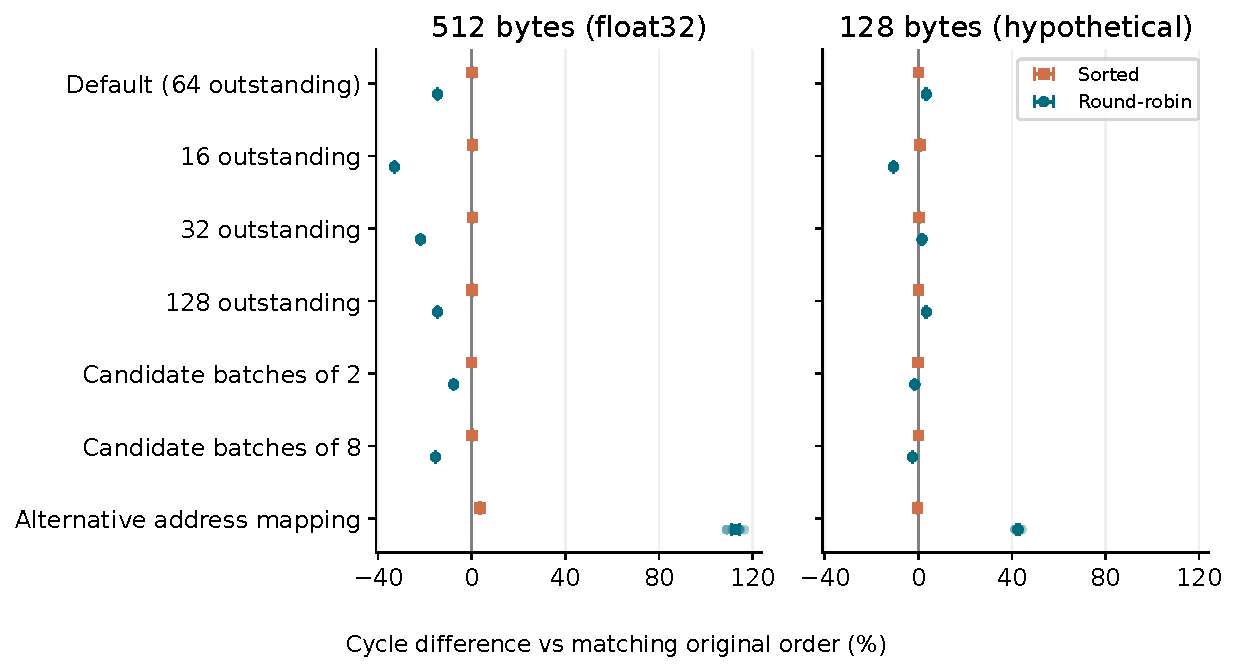
\includegraphics[width=\textwidth]{generated/scheduling_sensitivity.pdf}
\caption[How execution constraints change request ordering]{Scheduling differences against matching original-order BFS. Faint points are the ten split effects; larger markers and bars show their mean and paired 95\% interval. Both footprints use the same horizontal scale. The large alternative-mapper loss remains visible rather than being omitted to enlarge the default gain.}\label{fig:scheduling-sensitivity}
\end{figure}

Per-query savings, faster-query fractions and changes in the empirical 95th percentile are retained in Appendix~\ref{app:scheduling-detail}. They describe variation within each case and do not create additional independent repetitions. The result supports profiling a schedule for the execution configuration, which the next section evaluates with training queries.

\section{Does a training profile choose a useful schedule?}
\label{sec:profile-results}
Table~\ref{tab:profile-results} evaluates the fixed 50-query rule from Section~\ref{sec:profile-protocol}. Across 140 configuration/split choices, it selects original order \ProfileOriginalChoices{} times, sorting \ProfileSortedChoices{} times and round-robin \ProfileRRChoices{} times. Each chosen order is then evaluated on its matching held-out stream. The choice counts make clear whether a gain comes from selecting a different schedule or simply recovering a consistently useful fixed one. When original order is selected, the result reuses the baseline stream: its zero difference and zero-width interval are identities, not a statistical equivalence test for a deployed frontend with overhead.

\begin{table}[htbp]\centering\small
\caption[Training-selected schedules on held-out queries]{BFS placement, 50 calibration queries and 200 held-out queries per split. O/S/R counts denote original/sorted/round-robin choices across ten splits. Differences from original order are means with paired 95\% intervals; the oracle gap is the mean excess over the best fixed order chosen retrospectively for each held-out split. Lower is better.}\label{tab:profile-results}
\resizebox{\textwidth}{!}{\begin{tabular}{lrrrr}
\toprule
Condition & Bytes & Choices O/S/R & vs original (\%) & Oracle gap (\%) \\
\midrule
Default (64 outstanding) & 512 & 0/0/10 & -14.58 [-14.64, -14.51] & 0.000 \\
Default (64 outstanding) & 128 & 10/0/0 & +0.00 [+0.00, +0.00] & 0.000 \\
16 outstanding & 512 & 0/0/10 & -33.08 [-33.21, -32.94] & 0.000 \\
16 outstanding & 128 & 0/0/10 & -10.61 [-10.68, -10.54] & 0.000 \\
32 outstanding & 512 & 0/0/10 & -21.86 [-21.95, -21.78] & 0.000 \\
32 outstanding & 128 & 10/0/0 & +0.00 [+0.00, +0.00] & 0.000 \\
128 outstanding & 512 & 0/0/10 & -14.58 [-14.64, -14.51] & 0.000 \\
128 outstanding & 128 & 10/0/0 & +0.00 [+0.00, +0.00] & 0.000 \\
Candidate batches of 2 & 512 & 0/0/10 & -7.77 [-7.79, -7.76] & 0.000 \\
Candidate batches of 2 & 128 & 0/0/10 & -1.48 [-1.51, -1.46] & 0.000 \\
Candidate batches of 8 & 512 & 0/0/10 & -15.55 [-15.60, -15.50] & 0.000 \\
Candidate batches of 8 & 128 & 0/0/10 & -2.48 [-2.52, -2.43] & 0.000 \\
Alternative address mapping & 512 & 10/0/0 & +0.00 [+0.00, +0.00] & 0.000 \\
Alternative address mapping & 128 & 0/10/0 & -0.34 [-0.36, -0.33] & 0.000 \\
\bottomrule
\end{tabular}
}
\end{table}

The training choice matches the retrospectively best fixed order in \ProfileOracleMatches{} of 140 held-out configuration/split cases. The largest mean and single-split oracle gaps are \ProfileMaxMeanRegret\% and \ProfileMaxSplitRegret\%, with \ProfileOriginalRegressions{} aggregate regressions relative to original order. Each configuration receives the same choice across all ten training splits. Profiling therefore recovers a consistently useful fixed order in this matrix; these data do not show a need for per-query adaptation.

This is an observed result on the evaluated workload, not a guarantee for future queries. The policy was motivated by previously inspected outcomes, and its evaluation remains exploratory. A different query distribution could favour another order. Original order is one of the candidates, not a mathematical protection against held-out regression.

Aggregate gains can also coexist with slower individual queries. Table~\ref{tab:profile-query} retains the slower-query fraction and empirical 95th-percentile service change for the selected path under every setting. Under the alternative mapper at 128 bytes, 20.5--28.0\% of individual queries are slower across the ten splits, and the 95th-percentile change ranges from a 0.68\% reduction to a 0.38\% increase despite the aggregate saving. Small batches at 128 bytes also contain individual regressions. These are descriptive checks of the same query records; they are not additional independent trials or a bound on production tail latency.

\begin{figure}[htbp]\centering
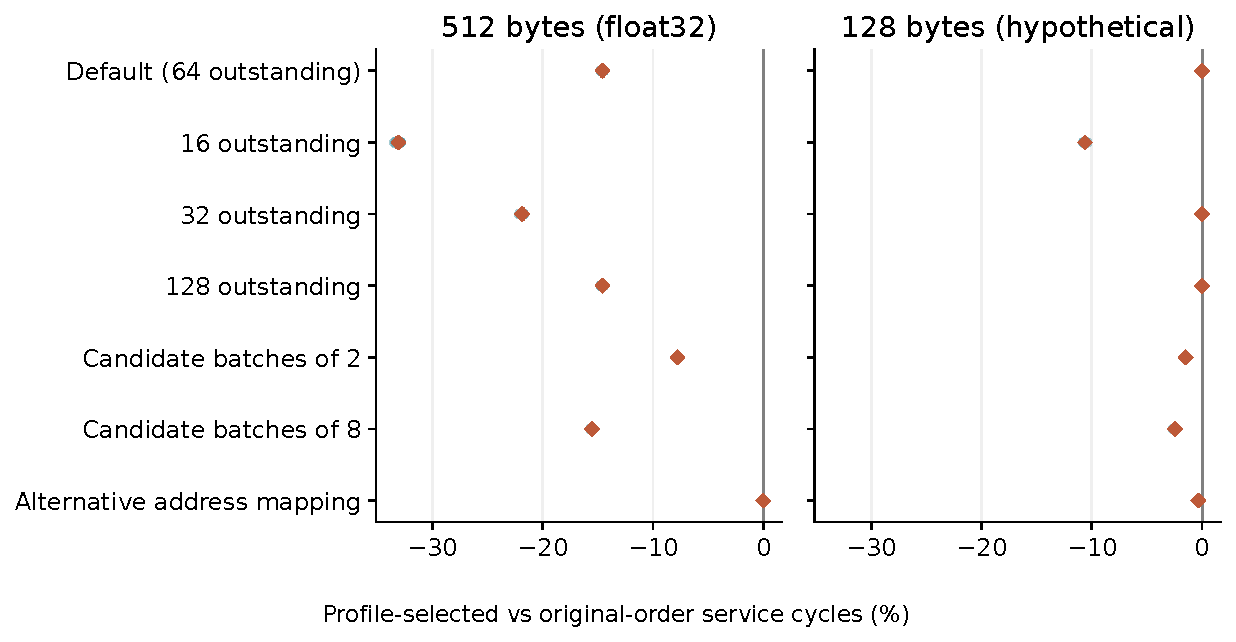
\includegraphics[width=\textwidth]{generated/profiled_fetch.pdf}
\caption[Held-out effect of the training-selected path]{Selected schedule versus original order under each matching configuration. Faint points show all ten split effects; diamonds and bars show means and paired 95\% intervals. Selection uses training cycles only. The footprint and one-setting-at-a-time restrictions are the same as in Figure~\ref{fig:scheduling-sensitivity}.}\label{fig:profiled-fetch}
\end{figure}

\subsection{Comparison with existing methods}
At default settings, Table~\ref{tab:profile-baselines} compares the selected BFS path with every fixed BFS schedule and the published placement routines under original-order bounded replay. The comparison to a fixed schedule is necessary: selecting round-robin does not improve on round-robin itself. Comparisons to RCM, Gorder and Porder change both placement and scheduling; they test the complete measured configurations. At 512 bytes, the selected path differs from Porder with original order by \ProfileVsPorderFloat\%; at the hypothetical 128-byte footprint, it uses original order and differs from Gorder by \ProfileVsGorderCompact\%. The proposal therefore complements the placement comparison without winning every baseline. These results do not establish that BFS plus profiling is optimal, or predict how a published placement would behave with the same selector.

\begin{table}[htbp]\centering\small
\caption[Profiled path versus measured baselines]{Default memory configuration and expansion boundaries. Mean paired cycle difference (\%) and 95\% interval across ten reference splits. Original, sorted and round-robin use BFS; RCM, Gorder and Porder use their respective placements and original order. The oracle is descriptive and uses held-out outcomes.}\label{tab:profile-baselines}
\begin{tabular}{lrr}
\toprule
Bytes & Comparator & Profiled path difference (\%) \\
\midrule
512 & Original & -14.58 [-14.64, -14.51] \\
512 & Sorted & -14.73 [-14.81, -14.66] \\
512 & Round-robin & +0.00 [+0.00, +0.00] \\
512 & Oracle & +0.00 [+0.00, +0.00] \\
512 & RCM & -14.44 [-14.53, -14.35] \\
512 & Gorder & -14.40 [-14.50, -14.31] \\
512 & Porder & -14.25 [-14.36, -14.14] \\
128 & Original & +0.00 [+0.00, +0.00] \\
128 & Sorted & -0.17 [-0.21, -0.12] \\
128 & Round-robin & -3.31 [-3.42, -3.20] \\
128 & Oracle & +0.00 [+0.00, +0.00] \\
128 & RCM & +0.47 [+0.38, +0.56] \\
128 & Gorder & +1.35 [+1.26, +1.44] \\
128 & Porder & +1.20 [+1.05, +1.35] \\
\bottomrule
\end{tabular}

\end{table}

The artifact also retains comparisons against every fixed order in every sensitivity condition in \texttt{results/profiled\_fetch\_summary.csv}. Published PIM systems are positioned by method and scope in Table~\ref{tab:related}; their end-to-end speedups cannot serve as numerical baselines for a trace-service percentage on different hardware and workloads.

\subsection{What the profile costs}
Calibration executes three 50-query streams per configuration, even though deployment uses only one schedule. Table~\ref{tab:profile-service} also gives absolute service for every setting: a larger percentage saving against a slower baseline does not establish that the whole configuration is faster. For example, the selected 512-byte path averages 41,316 service cycles per query at limit 16, compared with 34,008 at the default limit, despite its larger relative reduction. Appendix~\ref{app:profile-cost} reports that total service cost and the held-out saving per query separately. The experiment omits the cost of collecting a profile on the target, performing selection, storing the configuration key and executing the chosen order. A configuration with little or no service saving has correspondingly little room to recover those costs. Profiling is most relevant to a stable graph and workload that can reuse the choice; its application-level break-even point remains unmeasured.


\section{Construction cost and synthetic cross-check}
Across primary runs, mean index construction takes \MeanIndexSeconds{} s, collecting training traces takes \MeanTrainingSeconds{} s, and building the co-visitation model takes \MeanModelSeconds{} s on the execution host. Table~\ref{tab:cost} reports per-layout construction. The \QA{} layout time alone does not include its training and model stages. BFS requires graph traversal and memory for the mapping; it is not free. These shared-host observations are useful accounting, not hardware-independent performance predictions.
\begin{table}[htbp]\centering\caption[Layout construction cost]{Observed layout construction times for the primary float32 footprint. Shared-host wall-clock measurements; no performance-isolation claim.}\label{tab:cost}
\begin{tabular}{lr}
\toprule
Layout & Mean construction (s), 512 B \\
\midrule
Identity & 0.0000 \\
Random & 0.0009 \\
BFS & 0.0238 \\
Community & 0.9822 \\
Query-aware & 0.0285 \\
\bottomrule
\end{tabular}
\end{table}

The separate synthetic check uses 8,000 corpus vectors and a 2,000-query pool around the same 64 centroids, with 300 training and 150 test queries. Corpus and query generation share the centroids and are independent of the split seed. Its raw recall, layouts and timing results are retained under \texttt{results/synthetic}. This workload is useful for checking the pipeline, but a difference from SIFT cannot by itself identify whether graph structure, query distribution, training coverage or layout objectives caused it. Synthetic centroid proximity is not evidence that a particular real workload is uniformly clustered.

\chapter{Interpretation and threats to validity}
\section{Claims, evidence and boundaries}
\label{sec:claim-scope}
Table~\ref{tab:claim-scope} separates the conclusions established by this artifact from the stronger claims that require a different experiment. A negative result has a named intervention and baseline; a positive result has a measured service objective and an explicit execution boundary.

\begin{table}[htbp]\centering\small
\caption[What each result establishes]{A guide to the interpretation of the current evidence. All timing claims in this table concern simulated DRAM service.}\label{tab:claim-scope}
\begin{tabular}{>{\raggedright\arraybackslash}p{0.26\textwidth}>{\raggedright\arraybackslash}p{0.34\textwidth}>{\raggedright\arraybackslash}p{0.29\textwidth}}
\toprule
Claim & Supporting comparison & Boundary\\\midrule
A row-hit improvement can accompany a timing loss. & Identical-work microbenchmarks, query-aware/BFS contrasts and command accounting. & Does not imply that row reuse is generally harmful.\\
Established placements can outperform the local heuristic. & RCM, Gorder and Porder under matching flat and bounded replay. & Does not reproduce their cache-aware application benchmarks.\\
Interleaving available vector chunks can reduce service. & Original/sorted/round-robin on matching expansions, including paired and per-query effects. & Depends on footprint, mapping, available work and omitted overhead.\\
A training profile can guide the fetch schedule. & Fixed 50-query rule, held-out comparisons to every fixed order, oracle gaps and calibration cost. & Exploratory, one corpus and operating point; future-query gains are not guaranteed.\\
A configurable near-memory gather path merits implementation testing. & Conditional service savings and an explicit buffering/execution sketch. & No implemented accelerator, end-to-end speedup or energy result.\\\bottomrule
\end{tabular}
\end{table}

\section{Answers supported by the evidence}
\textbf{RQ1.} Access order changes both row classifications and service time in the controlled model. The direction of cycle improvement depends on concurrency: the default sequential stream has more hits and more cycles, whereas full sorting reduces cycles with one outstanding read. Presorting results are limited to the tested disjoint windows. Contiguous runs and valid placement perturbations characterise available locality; they do not demonstrate a reusable HNSW layout that creates the same runs.

\textbf{RQ2.} The initial flat-replay query-aware differences against BFS are \QADeltaFloat\% and \QADeltaCompact\% at the two footprints. Stronger published placements improve on that local heuristic in the reference comparison. With expansion boundaries, Porder gives \PorderBoundedFloat\% relative to BFS at 512 bytes; Gorder gives \GorderBoundedCompact\% at 128 bytes. Within-expansion round-robin on BFS changes cycles by \RoundRobinBFSMeanFloat\% and \RoundRobinBFSMeanCompact\% respectively. Address sorting changes them by \SortedBFSMeanFloat\% and \SortedBFSMeanCompact\% under those default settings. The profiled path compares these three orders using training queries only; Section~\ref{sec:profile-results} reports its held-out effect against every fixed order and the published placements. These are conditional positive alternatives and negative results with named baselines, not a general rejection of placement or scheduling.

\textbf{RQ3.} Footprint and the memory work made available to the controller materially affect the result. The prior controller study and the new phase boundaries test different assumptions: limiting outstanding transactions does not by itself withhold later graph discoveries. The construction tables separately report the selected graph variations. The scheduling sensitivity reverses the round-robin recommendation under changed request limits and address mapping. The 128-outstanding setting and candidate batches test additional, distinct constraints. The selector adapts to these measured configurations, but its short profile does not guarantee improvement on future queries. The one-setting-at-a-time matrix does not establish an optimal combination of every layout and schedule.

\section{Practical significance and an overhead budget}
\label{sec:overhead}
\textbf{Statistical significance} concerns the precision of an estimated effect under the sampling protocol. The flat-replay 512-byte query-aware/BFS interval excludes zero: \QADeltaFloat\% [\QALowFloat, \QAHighFloat]. That supports a nonzero conditional mean under the interval assumptions, without a family-wise or confirmatory claim.

\textbf{Practical significance} concerns whether the effect survives implementation cost and improves a useful system objective. The same placement difference saves approximately \SavedCyclesPerQuery{} controller cycles per query. On its own, this is weak justification for deploying an additional trained layout. The stronger default bounded comparison saves \RoundRobinBFSSavedFloat{} cycles per query for BFS round-robin at 512 bytes (\RoundRobinBFSMeanFloat\%); at 128 bytes its saved-cycle count is \RoundRobinBFSSavedCompact{} (\RoundRobinBFSMeanCompact\%), a regression. Address sorting saves \SortedBFSSavedFloat{} and \SortedBFSSavedCompact{} cycles at the two widths, also regressions. Table~\ref{tab:followup-schedules} reports the matching paired intervals. These are mean absolute service differences, rounded independently of percentages, and remain before scheduling or integration overhead.

\textbf{Architectural significance} concerns what the result teaches about a design choice. Even a small reversal shows why row-hit rate alone cannot choose a layout. The much larger scheduling contrast shows that the work exposed to a controller can matter more than the tested placement change. Its dependence on footprint, mapping and request capacity is a reason to expose and evaluate configurable fetch ordering; it does not establish a new accelerator's performance.

Consider an explicitly simplified additive model. Let $C$ be all shared non-memory work, $M_B$ and $M_Q$ the memory-service costs for BFS and query-aware layouts in the same units, and $H$ any extra per-query cost of the latter implementation:
\begin{align}
 T_B &= C+M_B, & T_Q &= C+M_Q+H.\\
 T_Q<T_B &\quad\Longleftrightarrow\quad H<M_B-M_Q.
\end{align}
Substituting the observed stream means gives an illustrative overhead allowance of about \SavedCyclesPerQuery{} controller cycles per query. It is not a measured CPU or PIM budget: real computation and memory may overlap, and graph dependencies change the memory schedule. The calculation makes the practical question explicit rather than assuming translation and integration are free.

For the default 512-byte scheduling comparison, the analogous allowance is \RoundRobinBFSSavedFloat{} service cycles per query. Extra dispatch, mapping accesses, buffer traffic, synchronisation and transfers must collectively fit within the retained saving. For two schedules on the same accelerator, only their \emph{additional} cost belongs in this difference; shared distance computation and transfers affect total execution time but must not be charged twice. If those extra operations consume half the allowance, approximately 2,901 controller-equivalent cycles remain per query before calibration. At or above the full allowance, the scheduling gain disappears in this additive example. These are cost thresholds, not measurements of the missing operations.

The artifact stores both mapping directions as 64-bit entries, requiring $16N$ bytes, or \MappingMiB{} MiB at $N=100{,}000$, before container overhead. An implementation might encode the mapping differently or rewrite neighbour IDs, but then must account for that representation, conversion and update work. Offline preprocessing also requires amortisation over a useful workload lifetime. Shared-host CPU seconds and simulated controller cycles cannot be mixed to produce a valid deployment break-even query count.

Equivalently, in that additive model let $f=M_B/(C+M_B)$ be the fraction of baseline time spent in the service being improved, $r=(M_B-M_Q)/M_B$ its fractional reduction, and $h=H/(C+M_B)$. The total-time reduction is $fr-h$. Even if an implementation retained a 14.58\% service reduction, an assumed $f=0.5$ and zero extra overhead would imply only a 7.29\% total-time reduction in this example. Neither $f$ nor $h$ is measured here, and overlap can invalidate the additive model. Consequently, no numerical end-to-end benefit is predicted.

\section{A PIM-oriented execution recommendation}
\label{sec:execution-sketch}
The measured mechanism is DRAM request scheduling and can matter to a CPU as well as to PIM. Its PIM relevance is a specific design decision: if a near-memory engine gathers vectors for HNSW distance evaluation, how should it expose the reads that are currently available? Moving computation closer to storage does not remove bank timing constraints. A placement that improves row reuse can still restrict useful overlap, and a frontend that interleaves chunks can help or hurt depending on the memory interface. This study establishes those conditional service effects, not an advantage unique to PIM.

\subsection{A concrete division of work and data}
Consider a host-controlled gather-and-distance design (Figure~\ref{fig:profile-execution}). Keep HNSW traversal, the visited set and the candidate/result queues on the host. Keep vectors and adjacency lists in memory addressable by a near-memory engine. The host reads a neighbour list, selects unvisited candidates and resolves their vector addresses. It sends a batch descriptor containing those addresses and original-order tags. A query vector is supplied once and retained near memory while that query runs. The engine gathers the batch, evaluates squared Euclidean distances and returns tagged distances; the host applies them in the original candidate order before choosing the next expansion.

This split is a proposed integration point, not an implemented platform. Vector gathering and per-candidate distance arithmetic are plausible near-memory operations because they consume resident arrays and return small results. Visited-set accesses, heap updates and graph control could also move to a programmable memory-side processor, but would require storage, synchronisation and a new execution evaluation. The present recommendation keeps them on the host to make that additional commitment explicit. Table~\ref{tab:pim-residency} summarises data residency and transfers.

\begin{table}[htbp]\centering\small
\caption[Data residency and transfers in the proposed PIM path]{One possible host-controlled gather-and-distance integration. Residency and transfers are design assumptions; only the recorded list and vector DRAM reads are timed by this thesis.}\label{tab:pim-residency}
\begin{tabular}{>{\raggedright\arraybackslash}p{0.22\textwidth}>{\raggedright\arraybackslash}p{0.31\textwidth}>{\raggedright\arraybackslash}p{0.36\textwidth}}
\toprule
Data & Proposed location & Movement or use\\\midrule
Vectors and adjacency & DRAM behind the near-memory engine & List IDs reach host control; candidate vectors feed local distance evaluation.\\
Query vector & Host and engine local storage & Send once per query per participating engine; reuse across candidate distances.\\
Visited set and search queues & Host & Updated after candidate discovery and ordered distance completion.\\
Node-to-slot mapping & Host in this example & Resolves IDs to vector addresses; mapping lookups are an additional cost.\\
Batch descriptors & Host to engine & Addresses, candidate identity/order tags and batch length.\\
Candidate data and results & Engine local storage & Buffer vector chunks or partial sums; return tagged distances to the host.\\\bottomrule
\end{tabular}
\end{table}

A gather-only engine that returns full vectors to host arithmetic still moves the vector payload across the host interface. Adding distance evaluation near memory is what could avoid that transfer. For a batch of $B$ candidates, the avoided payload would be $Bb$ bytes, replaced by descriptors and $B$ tagged distances, with query and neighbour-list transfers still required. This is byte accounting, not a bandwidth or energy result; protocol overhead, replication and repeated reads can alter total traffic. At 512 bytes the arithmetic uses the measured float32 representation. The hypothetical 128-byte experiment supplies no corresponding compressed-distance kernel or accuracy result.

\subsection{Dependencies and hardware requirements}
Candidate discovery must precede its vector requests. After a list arrives, reads for its available candidates can overlap, but the next graph expansion may depend on their distances. Request completion order must not change the order of search-state updates, stopping rules or ties. Reproducing distances also requires compatible numerical precision and reduction behaviour; preserving memory order alone cannot guarantee identical search on a different arithmetic unit. The following pseudocode expresses this dependency, with distance computation assigned to the engine and search updates to the host in the example above. It sketches the expansion stage; entry-vector evaluation and initial search-state setup are omitted.

\begin{lstlisting}
order = lookup_profile(configuration) or ORIGINAL
while search_needs_an_expansion():
    candidates = read_list_and_select_unvisited()
    for batch in consecutive_batches(candidates, B):
        addresses = resolve_vector_addresses(batch)
        chunks = make_native_reads(addresses, vector_bytes)
        for chunk in order_reads(chunks, order):
            submit_when_capacity_available(chunk)
        wait_for_batch_reads()
        for candidate in batch:  # original candidate order
            distance = compute_distance(candidate, query)
            update_search_state(candidate, distance)
\end{lstlisting}

Original order offers all chunks of one vector before offering the next vector's chunks; it does not wait for completion between vectors. Sorting orders the batch's chunk addresses. Round-robin offers chunk zero of every vector, then chunk one of every vector, and so on. A configuration profile selects between these established orders. Selection and fallback costs are discussed in Section~\ref{sec:profile-deployment}.

The target needs a programmable request frontend, several outstanding reads, completion tags, local storage for vectors or partial distances, query reuse and a distance unit with suitable arithmetic. To reproduce this study's intervention, it must expose ordering at the modelled 32-byte granularity and a compatible address mapping. A DMA interface that only accepts whole-vector transfers may hide that choice. A bank-local processor may also lack access to the cross-bank pool used by this single-channel experiment: partitioning, routing and query distribution would then need separate measurement. The assumed interface is not a claim about commercial UPMEM or every HBM-based PIM design~\cite{primer,upanns}.

This is an illustrative implementation sketch, not the measured program. The replay supplies the recorded candidates and addresses in advance and times their DRAM service. It does not execute candidate selection, address resolution, arithmetic, visited-state updates, result queues or local-buffer accesses. Those operations must be charged in a target implementation, along with any host/PIM transfers. Small-batch replay also adds drains without simulating the computation between them.

\begin{figure}[htbp]\centering
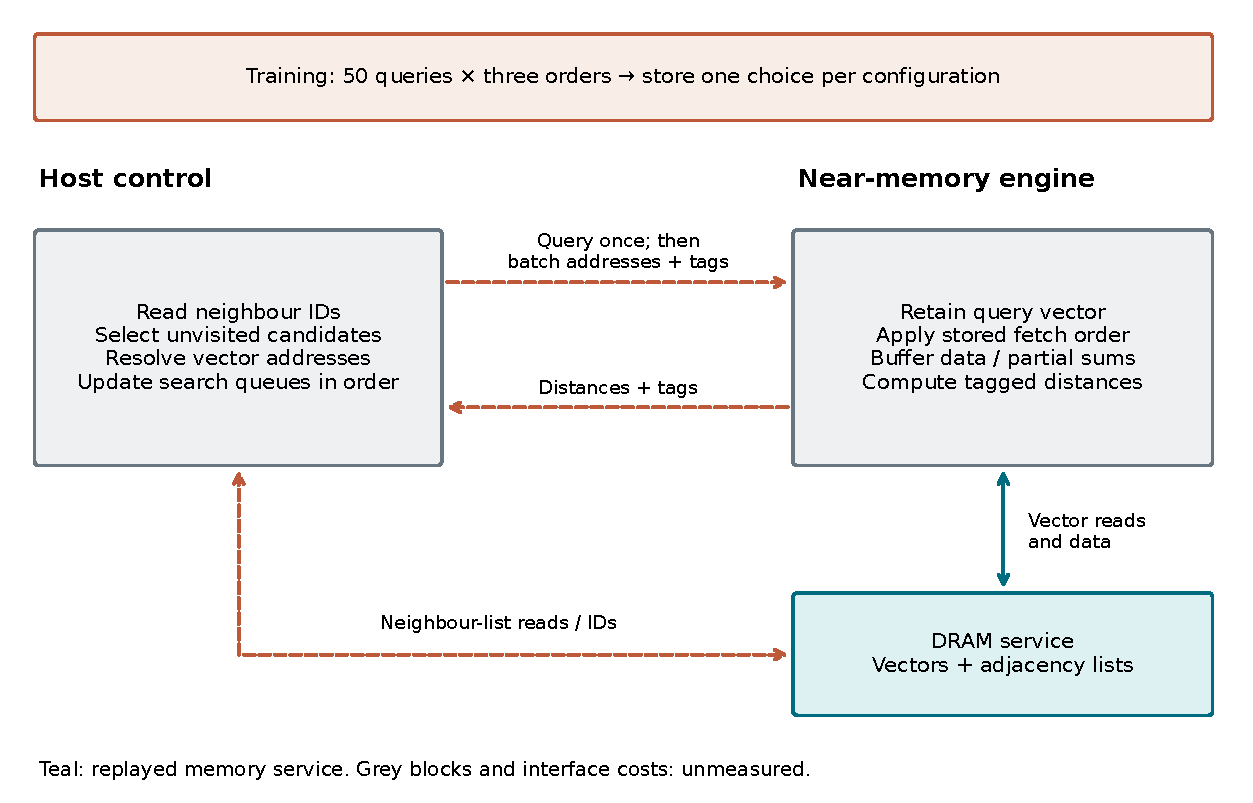
\includegraphics[width=\textwidth]{generated/profiled_fetch_execution.pdf}
\caption[Proposed host and near-memory execution boundary]{A host-controlled gather-and-distance design to evaluate. Training selects an order per configuration. Dashed arrows cross the host/engine boundary; the query is retained for reuse. Teal identifies the DRAM service included in replay, including neighbour-list reads. Grey control and computation blocks and all interface costs remain unmeasured. Returning distances instead of vectors requires the proposed distance unit.}\label{fig:profile-execution}
\end{figure}

For a straightforward full-vector buffer, $B$ candidates of $b$ bytes require at most $Bb$ payload bytes, plus addresses, query data and search state. At 512 bytes, batches of two and eight require 1 and 4 KiB respectively. A full 32-candidate base-layer list would require 16 KiB. These are storage calculations for this example; they are not measured scratch-memory traffic or a minimum for every design. A streaming distance kernel could use a different buffering strategy and would need its own evaluation.

\subsection{What the service result contributes to this design}
The measured saving supplies a target to test against: the default 512-byte BFS round-robin comparison leaves approximately \RoundRobinBFSSavedFloat{} simulated service cycles per query before extra costs. It compares two request orders inside the same memory model, not host execution with PIM execution. A host round trip at each expansion could dominate this saving. Conversely, keeping traversal near memory would change control and communication costs and possibly the available request overlap. Concurrent queries may already supply bank diversity, reducing the value of reordering one query. These possibilities explain why the service result guides an implementation experiment without predicting its application outcome.

For a complete accelerator, the next directly related experiment would implement this gather boundary with the target's native transfer granularity and local storage, then compare original, sorted and round-robin execution at the same recall and concurrency. Include a host-only HNSW baseline, the same accelerator with original-order fetch, and the profiled path with calibration cost reported separately. Measure end-to-end query latency and throughput, local-buffer occupancy, communication and distance-computation time. These controls would distinguish a scheduling benefit from an accelerator or batching benefit. The present evidence helps choose this experiment; it does not supply its unmeasured outcome.


\section{A decision path for a system designer}
The measurements suggest a concrete evaluation sequence.
\begin{enumerate}
\item \textbf{Establish comparable search work.} Fix the corpus, accuracy target and search settings. Check that a placement experiment preserves logical accesses and answers. If an encoding changes traversal or recall, evaluate it as a different search configuration.
\item \textbf{Measure the service objective.} Use completed cycles or actual application latency as appropriate, alongside traffic and locality. A proxy helps diagnose behaviour; it cannot select a winner by itself.
\item \textbf{Check the execution assumptions.} Decode the address map, identify the concurrency the application can really expose, and evaluate the relevant row policy. The same contiguous addresses can create different opportunities under another mapper.
\item \textbf{Choose using representative training work.} Compare fixed schedules under the actual batch and memory settings. Freeze the selected order before testing; preserve regressions and reprofile after relevant configuration changes.
\item \textbf{Compare benefit with implementation cost.} Include mapping accesses, storage movement, preprocessing, updates and workload drift on the target platform. The small default advantage here is a reason to measure these costs carefully.
\end{enumerate}
This is the useful engineering outcome of the study: a way to decide what evidence is needed before investing in a more complex layout. It does not prescribe one layout for every architecture.

\section{Internal validity}
The main threats addressed by the implementation are aliased storage, collision-producing placement, an independently rewritten search loop, layout construction inconsistent with footprint, cross-query metric transitions, and premature simulator termination. Input and mapping checks reject these failures before analysis. Raw data and generated tables make numerical accounting inspectable.

Remaining internal limits include the selected demand-access hooks and the modelling choice of a separate vector array with adjacency in another region. Keeping logical reads fixed isolates placement, but assumes that a physical integration would preserve the same algorithmic traversal. Mapping lookup traffic, cache effects and duplicate-read reuse could change the balance. The address-colocation metric intentionally omits adjacency and scheduling and must remain a diagnostic.

\section{Model and external validity}
Flat replay can expose future requests before a dependent HNSW execution discovers them. Expansion-bounded replay withholds later memory phases, but assumes candidate-vector overlap within a phase and adds no arithmetic time. It can therefore be more concurrent within an expansion and less concurrent across expansions than a particular implementation. Neither mode is a full execution model. Queries also drain sequentially: concurrent queries could expose bank diversity that changes the value of within-query reordering. Scratch memory, query-vector accesses, host/PIM transfers, index replication, processing-unit local memory, and energy are absent. Multiplying the observed cycle ratio by an assumed PIM bandwidth is not a measured PIM speedup.

The simulator models DRAM commands and timing rules, but the chosen preset contains estimates and is not validated here against a device trace. One configured HBM2 channel is not an entire HBM stack or a commercial PIM module. The alternate mapper and policies expand the conditional evidence without making it representative of all memory systems.

Only one real corpus prefix is evaluated. The four graph constructions test limited seed/order variation on that prefix; they do not test new datasets or eliminate source-order structure in the corpus. Ten-split intervals remain conditional on the primary graph, while the construction study reports its own finite observed variation. The synthetic clustered workload checks the pipeline on another generated input; it is not a second real-data validation.

The unevaluated dimensions have specific consequences. A new dataset or distance metric can change neighbourhood structure and which nodes queries visit. A different dimension or encoding changes transfer count and arithmetic cost; the 128-byte repacking isolates only transfer footprint while retaining float32 traversal. Changing HNSW connectivity or construction effort can change candidate-list sizes and graph paths. Changing search width or the requested recall target changes exploration, available vector groups and total work. Another graph-index family may expose different dependencies altogether. None of these effects is estimated by varying an index seed. Thus the evidence supports the named operating point and selected construction variations, not all HNSW settings, recall levels or graph-based ANN workloads.

\chapter{Conclusion}
This thesis contributes measured placement limits (C1), explained scheduling reversals (C2), and derived execution guidance (C3) for HNSW/HBM2. Its original output connects where identical search data live, when their reads become available and how the controller receives them. The locality--parallelism trade-off is established; these comparisons quantify its consequences for the evaluated graph search.

\textbf{RQ1: access order helps conditionally.} Controlled traces demonstrate a ranking reversal when concurrency changes. Fewer row operations can coexist with more no-command cycles. Contiguous runs and finite presorting expose opportunities within the tested grid; they do not establish a universal locality rule or a placement that creates those runs in HNSW.

\textbf{RQ2: useful alternatives depend on the comparison.} Under default flat replay, the query-aware placement is slightly faster than BFS at 512 bytes and slightly slower at the hypothetical 128-byte footprint. Published RCM, Gorder and Porder show that this local heuristic does not exhaust the placement opportunity. With expansion boundaries, round-robin on BFS changes cycles by \RoundRobinBFSMeanFloat\% and \RoundRobinBFSMeanCompact\%, respectively; address sorting is slower on average at both widths. Thus a natural locality-oriented choice can fail, while changing how available chunks are offered can help.

The proposal profiles three established orders on 50 training queries and freezes the choice for held-out service. It matches the best of those three fixed orders in all \ProfileOracleMatches{} cases: fourteen settings over ten splits of one workload. This exploratory observation is not a general success probability. A correctly chosen fixed order gives the same benefit without repeated calibration; individual-query regressions remain, and the selected default 128-byte path is slower than Gorder.

\textbf{RQ3: rankings do not survive every tested change.} Footprint, request limits and mapping can reverse recommendations; selected graph constructions reverse the small 128-byte placement result. These sensitivities establish conditional behaviour, not generality across datasets, recall targets or hardware.

Designers gain reproducible comparisons and acceptance criteria for a proposed gather-and-distance interface: test available-read order under the target mapper and concurrency, then charge incremental costs against the saving. A PIM implementation must replace replay phases with actual dependencies and measure computation, mapping, scheduling, local storage and communication at equal recall and concurrency. The artifact supplies service budgets, not a deployed accelerator or end-to-end speedup. Its DRAM findings also apply to host systems.

\appendix
\chapter{Artifact and reproduction}
\section{Authoritative files}
The thesis and companion sources use generated evidence from \texttt{results/}. The current matrix contains 2,069 replay records: 1,289 from the earlier checkpoint, 360 scheduling and 420 calibration runs. Calibration is training evidence, not independent held-out replication. Frozen design documents retain their checkpoint counts. Earlier PDFs and graphics remain under \texttt{archive/}; \nolinkurl{doc/RESULTS_PRESERVATION.md} identifies their status.

\section{Reproduction sequence}
The root README gives the starting commands; \nolinkurl{doc/REPRODUCIBILITY.md} supplies complete environment and data instructions. The maintained sequence is:
\begin{lstlisting}
python3 scripts/setup_published.py
make test
bash scripts/setup_ramulator.sh
python3 scripts/prepare_sift.py
make test-simulator
python3 scripts/experiments.py all --seeds 10 --jobs 2
python3 scripts/strengthen.py all --jobs 2
python3 scripts/followup.py --jobs 2
python3 scripts/scheduling.py --jobs 2
python3 scripts/profiled_fetch.py --jobs 2
make docs
\end{lstlisting}
Download the dataset HDF5 file to the path documented in the reproduction guide first. Setup verifies pinned archives; replay checks source identities, read accounting and sidecar hashes. Analysis rejects an incomplete matrix. Cache stamps are untracked, so a fresh clone runs simulations; subsequent runs can reuse validated local caches.

The reproduction guide maps claims to evidence and explains full reproduction and uncached spot checks. \nolinkurl{scripts/reproduce_replay.py} reconstructs HNSW demands and reruns the simulator; \nolinkurl{scripts/compare_reproduction.py} rejects differences in statistics or query/phase intervals against a separate reference. Input hashes, query IDs, lossless timing sidecars and figure provenance make the chain inspectable. Normal build cleanup preserves committed evidence.

\chapter{Supporting controls and implementation details}
\label{app:controls}
These experiments remain part of the evidence. They are grouped here so that the main results chapter follows the argument from controlled order effects to real search, stronger baselines and scheduling robustness.

\section{Contiguous runs, alignment, and placement quality}
Figure~\ref{fig:runs} separates hit-fraction behaviour from cycle behaviour. To summarise hit saturation on the finite grid, the threshold is the smallest tested run length for which that point and every larger tested point are within one percentage point of the best hit fraction in the same width/offset sweep. Table~\ref{tab:threshold} reports the resulting run \emph{bytes}. This is an empirical finite-grid summary, not a physical-law fit or a guarantee about untested run lengths.

\begin{figure}[htbp]\centering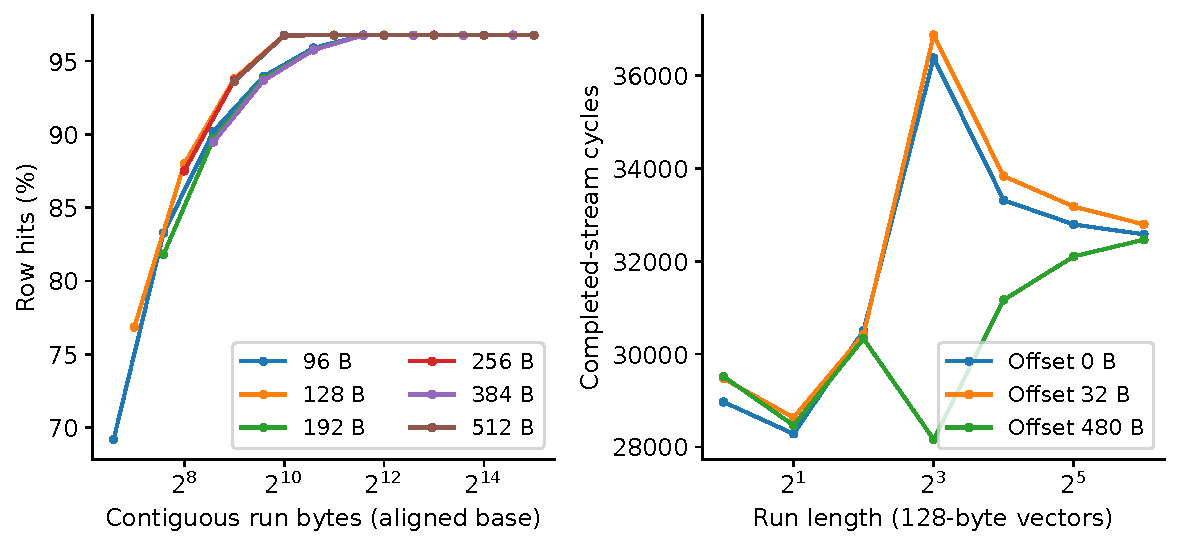
\includegraphics[width=\textwidth]{generated/run_sensitivity.pdf}
\caption[Contiguous runs and alignment]{Contiguous-run sensitivity to payload width and alignment. The left panel measures classified hits; the right panel shows that cycle behaviour requires separate examination.}\label{fig:runs}\end{figure}
\begin{table}[htbp]\centering\caption[Empirical run-byte thresholds]{Run-byte threshold for sustained hit fraction within one percentage point of the best tested point, by base offset. The threshold is conditional on this grid and configuration.}\label{tab:threshold}
\begin{tabular}{lrrr}
\toprule
Vector bytes & Offset 0 & Offset 32 & Offset 480 \\
\midrule
96 & 1536 & 3072 & 3072 \\
128 & 1024 & 4096 & 4096 \\
192 & 1536 & 3072 & 3072 \\
256 & 1024 & 4096 & 4096 \\
384 & 3072 & 3072 & 3072 \\
512 & 1024 & 4096 & 4096 \\
\bottomrule
\end{tabular}
\end{table}

The 1-KiB contiguous row span is independently established by address decoding. A saturation threshold can be larger, smaller in a particular grid, or affected by alignment and the controller's request mix. It should not be used to infer the row size after the fact. The alternate mapping experiments additionally change the bank opportunities associated with a contiguous address range. A predictive universal byte-budget rule is not established.

Figure~\ref{fig:quality} and Table~\ref{tab:quality} use only bijective layouts with identical address multisets. Reducing the fixed-slot fraction can move a vector within or across its original bank-row group, so the percentage is not a direct measurement of retained row locality. The curve describes this chosen corruption process. The experiment measures robustness to this specific perturbation. Translating a fixed-slot percentage into an acceptable engineering threshold would require a target cycle benefit and a preprocessing-cost model.
\begin{figure}[htbp]\centering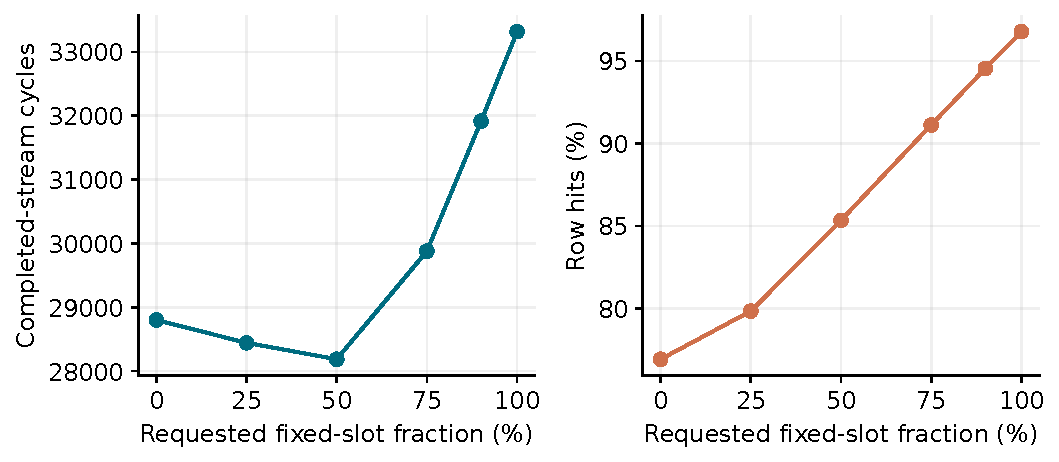
\includegraphics[width=\textwidth]{generated/quality.pdf}
\caption[Placement perturbation]{Valid fixed-slot-quality experiment. Each condition retains all 4,096 storage slots exactly once.}\label{fig:quality}\end{figure}
\begin{table}[htbp]\centering\caption[Placement-quality measurements]{Placement-quality results under the specified cyclic displacement process.}\label{tab:quality}
\begin{tabular}{lrr}
\toprule
Fixed slots (\%) & Cycles & Hit (\%) \\
\midrule
0 & 28801 & 76.92 \\
25 & 28443 & 79.84 \\
50 & 28186 & 85.34 \\
75 & 29880 & 91.11 \\
90 & 31915 & 94.54 \\
100 & 33316 & 96.77 \\
\bottomrule
\end{tabular}
\end{table}

\clearpage
\section{Controller and heuristic sensitivity}
\label{app:exploratory}
Figure~\ref{fig:sensitivity} compares layouts under the one-setting-at-a-time controller matrix. Each cell is a relative cycle difference against BFS in the \emph{same} condition and split. The heat map should not be read as independent evidence from ten repetitions for each cell. It shows how a finding can change when the issue model or bank mapping changes.

\begin{figure}[p]\centering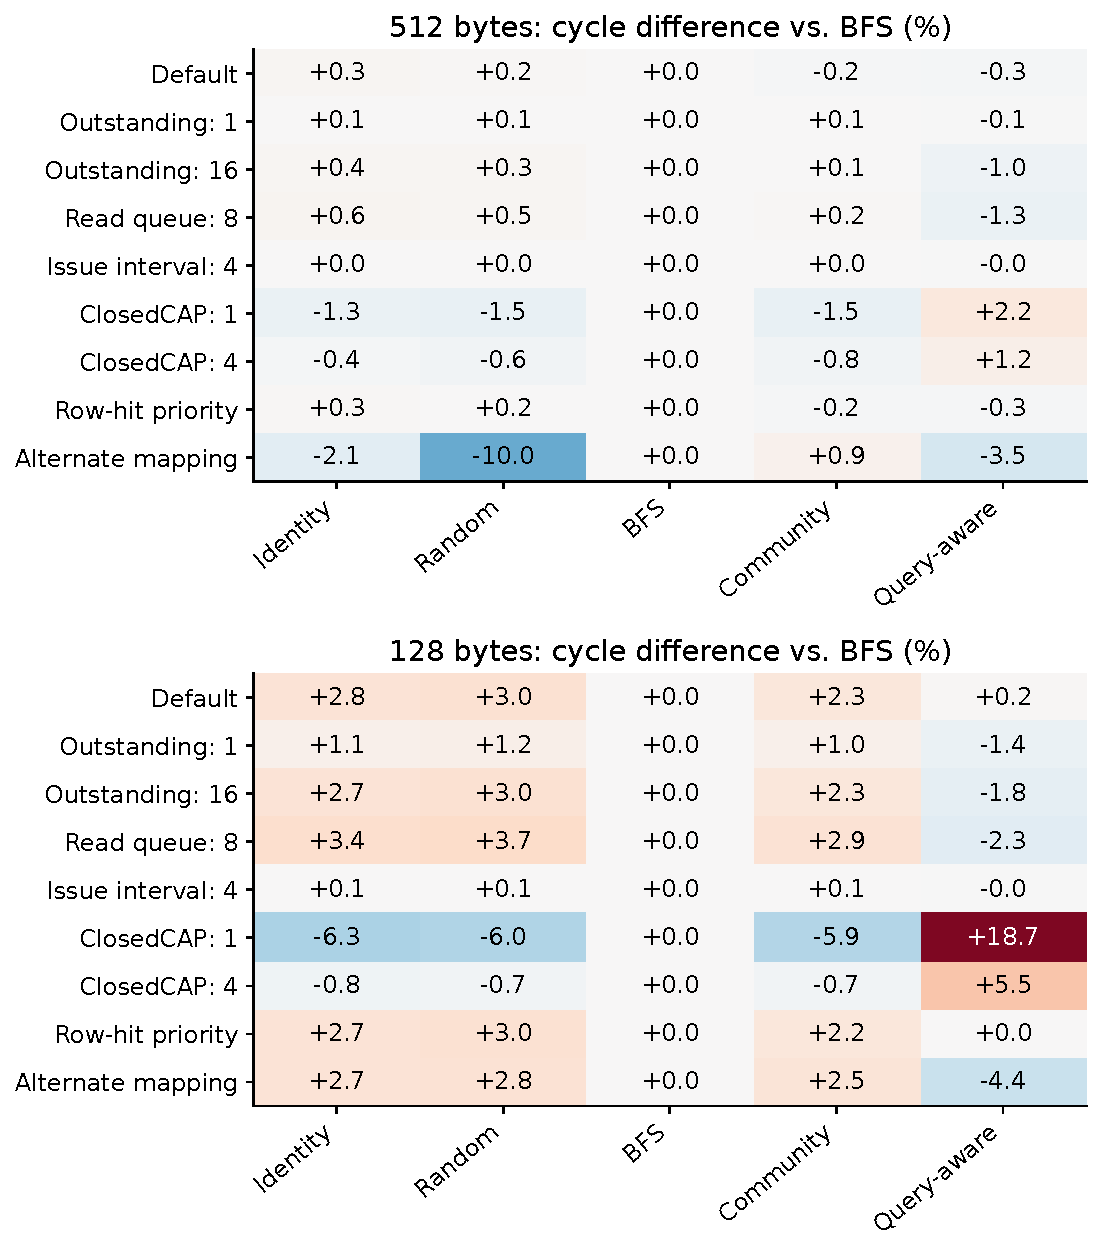
\includegraphics[width=\textwidth]{generated/sensitivity.pdf}
\caption[Exploratory controller sensitivity]{Split-one controller sensitivity. Values are cycle differences in percent against BFS; negative is fewer cycles. The two footprints use separately rebuilt layouts.}\label{fig:sensitivity}\end{figure}

The sensitivity matrix reverses some layout comparisons. For example, the workload-trained layout is faster than BFS with one outstanding request at both footprints, but slower under both capped policies. The alternate mapper favours it relative to BFS at both footprints in this split, although random placement is faster still for 512-byte vectors. These observations show dependence on the memory model; they are not additional ten-split estimates.

The cap-one policy and cap-four policy are explicitly different. In the controlled ordering traces, cap one gives sequential 146,441 cycles and random 33,798 cycles, while their classified hit fractions remain close to 50\%; cap four gives 63,333 and 29,708 cycles. These counters follow the simulator's scheduling-time classification and must not be interpreted as a guarantee that cap one produces zero classified hits. The much larger cycle separation demonstrates why a page-policy label or hit fraction is insufficient to predict service. The real-layout matrix supplies the relevant direct comparison; no claim that all placement benefit requires an open-page controller follows from the synthetic pair alone.

The ablations also change the sign of the comparison: the four-entry history loses to BFS at both widths, while 1,000 training queries give the workload-trained layout fewer cycles at both widths in this split. More training is not uniformly better for every footprint. These tests support examining the heuristic's objective and capacity rather than attributing all performance to static graph locality.

Table~\ref{tab:ablations} changes the heuristic's training and grouping parameters while retaining the test queries. Mean test vector-access coverage by the default training set is \MeanCoverage\%. Coverage here counts accesses whose node appeared in training, not the fraction of all corpus nodes or the fraction of learned edges shared with the graph. The ablations can reveal a limitation of this heuristic, but do not establish why every possible workload-trained placement would succeed or fail.

\begin{table}[htbp]\centering\small\caption[Training and grouping ablations]{Split-one heuristic ablations. Coverage is the fraction of test vector accesses to a node seen in training; model time excludes search collection and layout construction.}\label{tab:ablations}
\begin{tabular}{lrrrr}
\toprule
Condition & Bytes & $\Delta$ QA/BFS (\%) & Coverage (\%) & Model (s) \\
\midrule
train100 & 512 & -0.53 & 71.2 & 1.737 \\
train100 & 128 & +0.76 & 71.2 & 1.737 \\
train1000 & 512 & -0.26 & 99.7 & 24.494 \\
train1000 & 128 & -0.11 & 99.7 & 24.494 \\
window4 & 512 & +0.57 & 97.6 & 2.565 \\
window4 & 128 & +0.93 & 97.6 & 2.565 \\
window64 & 512 & -0.39 & 97.6 & 48.466 \\
window64 & 128 & +0.25 & 97.6 & 48.466 \\
block2048 & 512 & +0.24 & 97.6 & 11.249 \\
block2048 & 128 & +0.49 & 97.6 & 11.249 \\
\bottomrule
\end{tabular}
\end{table}


\section{Published-layout adapter and equivalence checks}
\label{app:adapters}
The source archive and extracted headers are hash-pinned. The adapter retains the supplied score updates and window-expiration condition \texttt{i > w+1}; that condition leaves the initial seed's contribution in place as later nodes expire. We report the supplied implementation rather than silently changing it to an idealised window. To make its weighted queue tractable at 100,000 nodes, an ordered set replaces the linked-list queue while preserving float score arithmetic and update-recency tie order. All three methods give byte-identical permutations to the untouched reference on 30 deterministic weighted test graphs (90 comparisons). This is a differential implementation check, not a proof for every possible graph. Timed preprocessing belongs to this adapted implementation.

\section{Scheduling: service variation within each case}
\label{app:scheduling-detail}
Table~\ref{tab:scheduling-query} supplements the total-cycle comparisons with original-query service. Positive saved cycles mean a reduction; negative percentile differences mean a lower empirical tail. Ranges cover the ten split-level summaries, rather than an interval estimated by treating all query records as independent. Complete paired effects for both sorted and round-robin orders remain in \texttt{results/scheduling\_pairs.csv} and \texttt{results/scheduling\_summary.csv}.

\begin{table}[htbp]\centering\small
\caption[Scheduling sensitivity by original query]{Round-robin versus matching original-order BFS. Saved cycles/query are averaged across ten splits; faster-query fractions and empirical 95th-percentile changes show the observed split range. Original-query intervals include inter-phase and inter-batch gaps.}\label{tab:scheduling-query}
\resizebox{\textwidth}{!}{\begin{tabular}{lrrrr}
\toprule
Condition & Bytes & Saved cycles/query & Faster queries (\%) & p95 change (\%) \\
\midrule
Default (64 outstanding) & 512 & +5,802 & 100.0--100.0 & -15.24 to -13.76 \\
Default (64 outstanding) & 128 & -541 & 6.0--15.0 & +4.25 to +5.95 \\
16 outstanding & 512 & +20,418 & 100.0--100.0 & -33.12 to -31.09 \\
16 outstanding & 128 & +2,106 & 100.0--100.0 & -11.09 to -9.00 \\
32 outstanding & 512 & +9,646 & 100.0--100.0 & -22.63 to -21.29 \\
32 outstanding & 128 & -261 & 20.5--31.0 & +0.63 to +3.86 \\
128 outstanding & 512 & +5,802 & 100.0--100.0 & -15.24 to -13.76 \\
128 outstanding & 128 & -541 & 6.0--15.0 & +4.25 to +5.95 \\
Candidate batches of 2 & 512 & +5,644 & 100.0--100.0 & -8.25 to -7.40 \\
Candidate batches of 2 & 128 & +559 & 92.5--96.0 & -2.54 to -1.11 \\
Candidate batches of 8 & 512 & +7,176 & 100.0--100.0 & -17.25 to -15.18 \\
Candidate batches of 8 & 128 & +500 & 87.0--95.0 & -3.59 to -1.72 \\
Alternative address mapping & 512 & -121,795 & 0.0--0.0 & +144.65 to +159.38 \\
Alternative address mapping & 128 & -25,309 & 0.0--0.0 & +56.29 to +59.74 \\
\bottomrule
\end{tabular}
}
\end{table}

\section{Calibration service and held-out savings}
\label{app:profile-cost}
Table~\ref{tab:profile-cost} reports the memory service spent on all three 50-query calibration runs, averaged over ten splits. The saving per held-out query uses the selected order and matching original-order BFS, including every phase gap. These figures share simulator units, but omit the operations and overlap of an actual execution. They therefore support a service-cost comparison, not a real deployment break-even calculation. Zero or negative held-out saving cannot pay for calibration in this simple accounting.

\begin{table}[htbp]\centering\small
\caption[Profiling cost and service saving]{Mean calibration service for 150 query replays per configuration, and mean saved cycles per held-out query relative to matching original order. Positive saved cycles are favourable. Calibration is performed once per profile; its reuse lifetime is unmeasured.}\label{tab:profile-cost}
\resizebox{\textwidth}{!}{\begin{tabular}{lrrr}
\toprule
Condition & Bytes & Calibration cycles & Saved cycles/query \\
\midrule
Default (64 outstanding) & 512 & 5,716,851 & +5,802 \\
Default (64 outstanding) & 128 & 2,404,776 & +0 \\
16 outstanding & 512 & 8,299,167 & +20,418 \\
16 outstanding & 128 & 2,895,259 & +2,106 \\
32 outstanding & 512 & 6,175,037 & +9,646 \\
32 outstanding & 128 & 2,440,817 & +0 \\
128 outstanding & 512 & 5,716,851 & +5,802 \\
128 outstanding & 128 & 2,404,776 & +0 \\
Candidate batches of 2 & 512 & 10,671,837 & +5,644 \\
Candidate batches of 2 & 128 & 5,652,508 & +559 \\
Candidate batches of 8 & 512 & 6,606,104 & +7,176 \\
Candidate batches of 8 & 128 & 3,025,606 & +500 \\
Alternative address mapping & 512 & 22,547,707 & +0 \\
Alternative address mapping & 128 & 10,246,779 & +202 \\
\bottomrule
\end{tabular}
}
\end{table}

\begin{table}[htbp]\centering\small
\caption[Per-query effects of the selected path]{Training-selected schedule versus matching original-order BFS. Entries show the range across ten splits of the fraction of queries with greater service time and the empirical 95th-percentile difference. Zero in a case selecting original order denotes the identical stream, not a separate confirmation of equivalence.}\label{tab:profile-query}
\resizebox{\textwidth}{!}{\begin{tabular}{lrrr}
\toprule
Condition & Bytes & Slower queries (\%) & p95 change (\%) \\
\midrule
Default (64 outstanding) & 512 & 0.0--0.0 & -15.24 to -13.76 \\
Default (64 outstanding) & 128 & 0.0--0.0 & +0.00 to +0.00 \\
16 outstanding & 512 & 0.0--0.0 & -33.12 to -31.09 \\
16 outstanding & 128 & 0.0--0.0 & -11.09 to -9.00 \\
32 outstanding & 512 & 0.0--0.0 & -22.63 to -21.29 \\
32 outstanding & 128 & 0.0--0.0 & +0.00 to +0.00 \\
128 outstanding & 512 & 0.0--0.0 & -15.24 to -13.76 \\
128 outstanding & 128 & 0.0--0.0 & +0.00 to +0.00 \\
Candidate batches of 2 & 512 & 0.0--0.0 & -8.25 to -7.40 \\
Candidate batches of 2 & 128 & 4.0--7.5 & -2.54 to -1.11 \\
Candidate batches of 8 & 512 & 0.0--0.0 & -17.25 to -15.18 \\
Candidate batches of 8 & 128 & 5.0--13.0 & -3.59 to -1.72 \\
Alternative address mapping & 512 & 0.0--0.0 & +0.00 to +0.00 \\
Alternative address mapping & 128 & 20.5--28.0 & -0.68 to +0.38 \\
\bottomrule
\end{tabular}
}
\end{table}

Table~\ref{tab:profile-service} provides absolute service means across all seven configurations. It prevents a favourable percentage against a slower configuration-specific baseline from being mistaken for a faster overall configuration. Lower outstanding capacity and smaller batches change the original-order service time as well as the gain from scheduling. The measured times still omit the computation and buffer constraints that would decide a deployed configuration.

\begin{table}[htbp]\centering\small
\caption[Absolute service across execution configurations]{Original and training-selected BFS service per held-out query, averaged across ten splits. Only the named setting changes from the default. These are simulated service means, not application latencies.}\label{tab:profile-service}
\resizebox{\textwidth}{!}{\begin{tabular}{lrrr}
\toprule
Condition & Bytes & Original cycles/query & Selected cycles/query \\
\midrule
Default (64 outstanding) & 512 & 39,811 & 34,008 \\
Default (64 outstanding) & 128 & 15,768 & 15,768 \\
16 outstanding & 512 & 61,734 & 41,316 \\
16 outstanding & 128 & 19,853 & 17,747 \\
32 outstanding & 512 & 44,116 & 34,471 \\
32 outstanding & 128 & 16,095 & 16,095 \\
128 outstanding & 512 & 39,811 & 34,008 \\
128 outstanding & 128 & 15,768 & 15,768 \\
Candidate batches of 2 & 512 & 72,625 & 66,981 \\
Candidate batches of 2 & 128 & 37,662 & 37,103 \\
Candidate batches of 8 & 512 & 46,150 & 38,974 \\
Candidate batches of 8 & 128 & 20,197 & 19,697 \\
Alternative address mapping & 512 & 108,034 & 108,034 \\
Alternative address mapping & 128 & 59,417 & 59,215 \\
\bottomrule
\end{tabular}
}
\end{table}


\chapter{Terminology}
\label{ch:terms}
\section{Search and memory}
\begin{longtable}{p{0.27\textwidth}p{0.64\textwidth}}\toprule
Term & Meaning in this thesis\\\midrule\endhead
ANN / ANNS & Approximate nearest neighbour search: retrieve close items while allowing some exact neighbours to be missed.\\
HNSW & Hierarchical Navigable Small World: a graph index whose upper layers guide a search toward promising regions.\\
Corpus / query & The stored vectors / the vector used to search for close stored items.\\
Recall@$k$ & The fraction of exact top-$k$ IDs recovered by an approximate search.\\
BFS & Breadth-first search; here, a graph traversal used to choose storage order.\\
Adjacency list & The stored neighbour IDs of a graph node.\\
DRAM / HBM & Dynamic random-access memory / high-bandwidth memory, a stacked DRAM technology.\\
Bank / row buffer & A DRAM subdivision with separate row state / its currently open row.\\
ACT / PRE / RD & Commands to activate (open), precharge (close), and read a row.\\
Address mapper & The rule assigning an address to channel, bank, row and column fields.\\
Outstanding read & A submitted request whose completion has not yet arrived.\\
FRFCFS & First-ready, first-come-first-served scheduling; the exact implementation determines priorities.\\
KiB / MiB & $2^{10}$ / $2^{20}$ bytes; different from decimal kB / MB.\\
Seed & An input that makes a pseudo-random procedure reproducible; its meaning depends on which procedure is varied.\\
\bottomrule
\end{longtable}
\clearpage
\section{Layouts, replay and evidence}
\begin{longtable}{p{0.27\textwidth}p{0.64\textwidth}}\toprule
Term & Meaning in this thesis\\\midrule\endhead
Logical trace & Ordered vector/list demands identified by node and query, before assigning physical addresses.\\
Vector layout & A bijection from logical nodes to dense storage slots.\\
Graph reordering & A memory-layout/graph relabelling optimisation in the cited literature; distinct from sorting pending request records.\\
RCM & Reverse Cuthill--McKee: a degree-ordered graph traversal whose order is reversed for placement.\\
Gorder / Porder & Published graph-reordering methods using structural relationships / traversal-weighted relationships.\\
Flat replay & Offers a known trace under the transaction limit, without draining between graph expansions.\\
Expansion phase & A list payload or its candidate-vector group; all reads finish before the next phase issues.\\
Round-robin & Offers one transaction from each available vector in turn, then repeats for their next chunks.\\
Request presorting & Stable address sorting within disjoint batches of an already known read stream.\\
Transaction & One native 32-byte read in the evaluated HBM2 configuration.\\
Row hit & A request classification made by the pinned simulator/controller; distinct from the flat same-block proxy.\\
Same-block fraction & A specified within-query vector-start colocation statistic, without a bank/scheduler model.\\
Stream cycles & Controller cycles through the final read completion under the frontend assumptions.\\
Footprint sensitivity & Repacking the same float32 traversal with a different modelled vector payload.\\
Paired interval & An interval calculated from layout differences on matching split conditions.\\
PIM speedup & End-to-end comparison involving a specified PIM system and baseline; not measured here.\\\bottomrule
\end{longtable}
\clearpage\addcontentsline{toc}{chapter}{Bibliography}
\begingroup\raggedright
\begin{thebibliography}{99}
\bibitem{hnsw} Y. A. Malkov and D. A. Yashunin, ``Efficient and robust approximate nearest neighbor search using hierarchical navigable small world graphs,'' \emph{IEEE Transactions on Pattern Analysis and Machine Intelligence}, vol. 42, no. 4, pp. 824--836, 2020. \url{https://doi.org/10.1109/TPAMI.2018.2889473}.
\bibitem{pq} H. J\'egou, M. Douze, and C. Schmid, ``Product quantization for nearest neighbor search,'' \emph{IEEE Transactions on Pattern Analysis and Machine Intelligence}, vol. 33, no. 1, pp. 117--128, 2011. \url{https://doi.org/10.1109/TPAMI.2010.57}.
\bibitem{primer} O. Mutlu, S. Ghose, J. G\'omez-Luna, and R. Ausavarungnirun, ``A modern primer on processing in memory,'' in \emph{Emerging Computing: From Devices to Systems}, Springer, 2022. \url{https://arxiv.org/abs/2012.03112}.
\bibitem{ramulator} H. Luo et al., ``Ramulator 2.0: A modern, modular, and extensible DRAM simulator,'' \emph{IEEE Computer Architecture Letters}, vol. 23, no. 1, pp. 112--116, 2024. \url{https://doi.org/10.1109/LCA.2023.3333759}.
\bibitem{ramsource} CMU-SAFARI, \emph{Ramulator2 source (Ramulator 2.1 implementation)}, revision \texttt{7bead6cb7c4b} (full revision in link), inspected 9 November 2026. \url{https://github.com/CMU-SAFARI/ramulator2/tree/7bead6cb7c4b03e095c6d4769ae3181a8e0bf6da}.
\bibitem{hnswlib} nmslib contributors, \emph{hnswlib: Header-only C++/Python library for fast approximate nearest neighbors}. Vendored source and observer patch identified in the accompanying artifact. \url{https://github.com/nmslib/hnswlib}.
\bibitem{annbench} M. Aum\"uller, E. Bernhardsson, and A. Faithfull, ``ANN-Benchmarks: A benchmarking tool for approximate nearest neighbor algorithms,'' \emph{Information Systems}, vol. 87, Art. no. 101374, 2020. \url{https://doi.org/10.1016/j.is.2019.02.006}. Dataset mirror: \url{https://ann-benchmarks.com/sift-128-euclidean.hdf5}.
\bibitem{coleman} B. Coleman, S. Segarra, A. Smola, and A. Shrivastava, ``Graph reordering for cache-efficient near neighbor search,'' \emph{Advances in Neural Information Processing Systems}, vol. 35, 2022. Published paper and supplementary implementation: \url{https://proceedings.neurips.cc/paper_files/paper/2022/hash/fb44a668c2d4bc984e9d6ca261262cbb-Abstract-Conference.html}.
\bibitem{cuthill} E. Cuthill and J. McKee, ``Reducing the bandwidth of sparse symmetric matrices,'' in \emph{Proceedings of the 1969 24th National Conference}, pp. 157--172, 1969. \url{https://doi.org/10.1145/800195.805928}.
\bibitem{gorder} H. Wei, J. X. Yu, C. Lu, and X. Lin, ``Speedup graph processing by graph ordering,'' in \emph{Proceedings of the 2016 International Conference on Management of Data}, pp. 1813--1828, 2016. \url{https://doi.org/10.1145/2882903.2915220}.
\bibitem{diskann} S. Jayaram Subramanya, F. Devvrit, H. V. Simhadri, R. Krishnaswamy, and R. Kadekodi, ``DiskANN: Fast accurate billion-point nearest neighbor search on a single node,'' \emph{Advances in Neural Information Processing Systems}, 2019. \url{https://github.com/microsoft/DiskANN}.
\bibitem{drim} M. Chen et al., ``DRIM-ANN: An approximate nearest neighbor search engine based on commercial DRAM-PIMs,'' \emph{SC}, 2025. \url{https://doi.org/10.1145/3712285.3759801}; preprint \url{https://arxiv.org/abs/2410.15621}.
\bibitem{upanns} S. Chen, A. C. Zhou, Y. Shi, Y. Li, and X. Yao, ``UpANNS: Enhancing billion-scale ANNS efficiency with real-world PIM architecture,'' \emph{SC}, 2025. \url{https://doi.org/10.1145/3712285.3759777}; preprint \url{https://arxiv.org/abs/2410.23805}.
\bibitem{pimann} P. Wu, M. Xie, E. Zhao, D. Zhang, J. Wang, X. Liang, K. Ren, and Y. Chai, ``Turbocharge ANNS on real processing-in-memory by enabling fine-grained per-PIM-core scheduling,'' \emph{USENIX Annual Technical Conference}, 2025. \url{https://www.usenix.org/conference/atc25/presentation/wu-puqing}.
\bibitem{pimcqg} S. Chen, Y. Li, Y. Chen, M. Deng, J. Meng, and A. C. Zhou, ``PIMCQG: Co-designing billion-scale graph-based approximate nearest neighbor search for processing-in-memory,'' arXiv:2605.25522v2, 3 November 2026. The public record states acceptance at SC26; checked 10 November 2026. \url{https://arxiv.org/abs/2605.25522}.
\bibitem{student} Student, ``The probable error of a mean,'' \emph{Biometrika}, vol. 6, no. 1, pp. 1--25, 1908. \url{https://doi.org/10.1093/biomet/6.1.1}.
\end{thebibliography}

\endgroup
\end{document}
